% Chapter 12: Spectral analysis
% Time Series Analysis -- Bachelor's programmes Economic Informatics and Economic Cybernetics, Bucharest University of Economic Studies
% GENERATED by latex/build_chapter12.py -- edit the generator, not this file.

\newcommand{\coursename}{Time Series Analysis}
% Preambul comun TSA -- Serii de timp / Time Series Analysis (Beamer, 16:9)
% Același design ca MFM și SFM (preluat din SFM, 5 octombrie 2026). Înainte de % Preambul comun TSA -- Serii de timp / Time Series Analysis (Beamer, 16:9)
% Același design ca MFM și SFM (preluat din SFM, 5 octombrie 2026). Înainte de % Preambul comun TSA -- Serii de timp / Time Series Analysis (Beamer, 16:9)
% Același design ca MFM și SFM (preluat din SFM, 5 octombrie 2026). Înainte de \input{../../latex/preamble} se definește
%   \newcommand{\coursename}{Time Series Analysis}      (EN)
%   \newcommand{\coursename}{Serii de timp}       (RO)  și  \def\tsalang{ro}
% Fișierele .tex se află în EN/Courses, EN/Seminars, RO/Cursuri, RO/Seminarii (două niveluri sub rădăcină).
% Deck-urile sînt generate de latex/build_chapterN.py / build_seminarN.py (vezi latex/tsa_build.py).

\documentclass[9pt, aspectratio=169, t]{beamer}
\providecommand{\coursename}{Time Series Analysis}

% Ensure content fits on slides
\setbeamersize{text margin left=8mm, text margin right=8mm}
% Smaller institute font (title page)
\setbeamerfont{institute}{size=\footnotesize}

%=============================================================================
% THEME AND STYLE CONFIGURATION
%=============================================================================
\usetheme{default}
% Using default theme for clean header/footer control

% Color Palette (matching Redispatch PDF)
\definecolor{MainBlue}{RGB}{26, 58, 110}
\definecolor{AccentBlue}{RGB}{26, 58, 110}
\definecolor{IDAred}{RGB}{205, 0, 0}
\definecolor{DarkGray}{RGB}{51, 51, 51}
\definecolor{MediumGray}{RGB}{128, 128, 128}
\definecolor{LightGray}{RGB}{248, 248, 248}
\definecolor{VeryLightGray}{RGB}{235, 235, 235}
\definecolor{KeynoteGray}{RGB}{218, 218, 218}
\definecolor{SectionGray}{RGB}{120, 120, 120}
\definecolor{FooterGray}{RGB}{100, 100, 100}
\definecolor{Crimson}{RGB}{220, 53, 69}
\definecolor{Forest}{RGB}{46, 125, 50}
\definecolor{Amber}{RGB}{181, 133, 63}
\definecolor{Orange}{RGB}{230, 126, 34}
\definecolor{Purple}{RGB}{142, 68, 173}

% Gradient background (exact Keynote 315° gradient: white to RGB 218,218,218)
\setbeamertemplate{background}{%
    \begin{tikzpicture}[remember picture, overlay]
        \shade[shading=axis, shading angle=315,
        top color=white, bottom color=KeynoteGray]
        (current page.south west) rectangle (current page.north east);
    \end{tikzpicture}%
}
% Fallback solid color for compatibility
\setbeamercolor{background canvas}{bg=}

\setbeamercolor{palette primary}{bg=MainBlue, fg=white}
\setbeamercolor{palette secondary}{bg=MainBlue!85, fg=white}
\setbeamercolor{palette tertiary}{bg=MainBlue!70, fg=white}
\setbeamercolor{structure}{fg=MainBlue}
\setbeamercolor{title}{fg=IDAred}
\setbeamercolor{frametitle}{fg=IDAred, bg=}
\setbeamercolor{block title}{bg=MainBlue, fg=white}
\setbeamercolor{block body}{bg=VeryLightGray, fg=DarkGray}
\setbeamercolor{block title alerted}{bg=Crimson, fg=white}
\setbeamercolor{block body alerted}{bg=Crimson!8, fg=DarkGray}
\setbeamercolor{block title example}{bg=Forest, fg=white}
\setbeamercolor{block body example}{bg=Forest!8, fg=DarkGray}
\setbeamercolor{item}{fg=MainBlue}

% Footer colors (override Madrid theme blue)
\setbeamercolor{author in head/foot}{fg=FooterGray, bg=}
\setbeamercolor{title in head/foot}{fg=FooterGray, bg=}
\setbeamercolor{date in head/foot}{fg=FooterGray, bg=}
\setbeamercolor{section in head/foot}{fg=FooterGray, bg=}
\setbeamercolor{subsection in head/foot}{fg=FooterGray, bg=}

% Bullet styles (apply everywhere including blocks)
\setbeamertemplate{itemize item}{\color{MainBlue}$\boxdot$}
\setbeamertemplate{itemize subitem}{\color{MainBlue}$\blacktriangleright$}
\setbeamertemplate{itemize subsubitem}{\color{MainBlue}\tiny$\bullet$}
\setbeamertemplate{itemize/enumerate body begin}{\normalsize}
\setbeamertemplate{itemize/enumerate subbody begin}{\normalsize}

% Item spacing - compact style
\setlength{\leftmargini}{10pt}       % Level 1: minimal indent
\setlength{\leftmarginii}{10pt}      % Level 2: minimal additional indent
% Compact list spacing (zero extra space before/after lists in blocks)
\makeatletter
\def\@listi{\leftmargin\leftmargini \topsep 0pt \parsep 0pt \itemsep 0pt}
\def\@listii{\leftmargin\leftmarginii \topsep 0pt \parsep 0pt \itemsep 0pt}
\makeatother

\setbeamertemplate{navigation symbols}{}

%=============================================================================
% CUSTOM HEADLINE
%=============================================================================
\setbeamertemplate{headline}{%
    \vskip10pt%
    \hbox to \paperwidth{%
        \hskip0.5cm%
        {\small\color{FooterGray}\renewcommand{\hyperlink}[2]{##2}\insertsectionhead}%
        \hfill%
        \textcolor{FooterGray}{\small\insertframenumber}%
        \hskip0.5cm%
    }%
    \vskip4pt%
    {\color{FooterGray}\hrule height 0.4pt}%
}

%=============================================================================
% CUSTOM FOOTER
%=============================================================================
\usepackage{fontawesome5}

\setbeamertemplate{footline}{%
    {\color{FooterGray}\hrule height 0.4pt}%
    \vskip4pt%
    \hbox to \paperwidth{%
        \hskip0.5cm%
        \textcolor{FooterGray}{\small\coursename}%
        \hfill%
        \raisebox{-0.1em}{%
            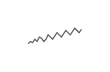
\begin{tikzpicture}[x=0.08em, y=0.08em, line width=0.4pt]
                \draw[FooterGray] (0,3) -- (1,4) -- (2,3.5) -- (3,5) -- (4,4) -- (5,6) -- (6,5.5) -- (7,4) -- (8,5) -- (9,7) -- (10,6) -- (11,5) -- (12,6.5) -- (13,8) -- (14,7) -- (15,6) -- (16,7.5) -- (17,9) -- (18,8) -- (19,7) -- (20,8.5) -- (21,10) -- (22,9) -- (23,8) -- (24,9.5);
            \end{tikzpicture}%
        }%
        \hskip0.5cm%
    }%
    \vskip6pt%
}

%=============================================================================
% PACKAGES
%=============================================================================
\usepackage[utf8]{inputenc}
\DeclareUnicodeCharacter{03B1}{\ensuremath{\alpha}}
\usepackage[T1]{fontenc}
\usepackage{amsmath, amssymb, amsthm}
\usepackage{mathtools}
\usepackage{bm}
\usepackage{tikz}
\usetikzlibrary{arrows.meta, positioning, shapes, calc, decorations.pathreplacing, shadings}
\usepackage{booktabs}
\usepackage{multirow}
\usepackage{array}
\usepackage{graphicx}
\usepackage{animate}
\usepackage{hyperref}
\usepackage{colortbl}
\usepackage{listings}
\lstset{language=Python, basicstyle=\ttfamily\scriptsize, keywordstyle=\color{MainBlue}\bfseries,
  commentstyle=\color{Forest}, stringstyle=\color{Crimson}, breaklines=true,
  frame=none, backgroundcolor=\color{VeryLightGray}, xleftmargin=2mm}
\hypersetup{colorlinks=true, linkcolor=MainBlue, urlcolor=MainBlue}
\graphicspath{{../../logos/}{../../charts/}{../../photos/}}
\usepackage{xcolor}
\hfuzz=2pt  % Suppress tiny overfull warnings (<2pt)
\vfuzz=2pt  % Suppress tiny vertical overfull warnings (<2pt)
% \mathrm in the sans-serif family of the slides (beamer resets \mathrm to the serif family at \begin{document};
% this hook runs after beamer's, so WN, Var, RMSE, ... in formulas match the surrounding text)
% Bold vectors and matrices in the same sans-serif family: \mathbf{A} in sans bold (beamer's own \mathbf came out in
% medium weight), and the bold upright Greek capitals of \boldsymbol / \bm (\bSigma, \bPhi, \boldsymbol{\Theta}) in
% cmss bold: bm.sty fixes its "boldoperators" font when it is loaded (serif cmbx), before beamer switches the
% operators to cmss, so it is reset here.
\AtBeginDocument{%
  \SetMathAlphabet{\mathrm}{normal}{\encodingdefault}{\sfdefault}{\mddefault}{n}%
  \SetMathAlphabet{\mathrm}{bold}{\encodingdefault}{\sfdefault}{bx}{n}%
  \SetMathAlphabet{\mathbf}{normal}{\encodingdefault}{\sfdefault}{bx}{n}%
  \SetMathAlphabet{\mathbf}{bold}{\encodingdefault}{\sfdefault}{bx}{n}%
  \SetSymbolFont{boldoperators}{normal}{OT1}{cmss}{bx}{n}%
  \SetSymbolFont{boldoperators}{bold}{OT1}{cmss}{bx}{n}}

%=============================================================================
% QUANTLET COMMANDS
%   \quantlet{<displayed name>}{<url>}       (generic, compatible with the older TSA decks)
%   \tsaquantlet{Ch_05}{TSA_ch5_garch}       -> https://github.com/danpele/Time-Series-Analysis/tree/main/Quantlets/Ch_05/TSA_ch5_garch
%   \qlurl{<folder>} is defined per chapter by the generator (Quantlets/Ch_NN/<folder>)
%=============================================================================
\newcommand{\tsarepo}{https://github.com/danpele/Time-Series-Analysis}
\newcommand{\tsaqlbase}{https://github.com/danpele/Time-Series-Analysis/tree/main/Quantlets}
\newcommand{\quantlet}[2]{%
    \hfill\href{#2}{%
        \raisebox{-0.15em}{
\includegraphics[height=0.7em]{ql_logo.png}}%
        \textcolor{MainBlue}{\tiny\ #1}%
    }%
}
\newcommand{\tsaquantlet}[2]{\quantlet{\detokenize{#2}}{\tsaqlbase/#1/#2}}

%=============================================================================
% NOTEBOOKS (Google Colab)
%   \colaburl{notebooks/EN/chapter5_seminar_notebook.ipynb} -> the Colab link of a file in the TSA repo
%   \nb: the chapter notebook (each seminar deck redefines it with \renewcommand)
%=============================================================================
\newcommand{\colaburl}[1]{https://colab.research.google.com/github/danpele/Time-Series-Analysis/blob/main/#1}
\newcommand{\nb}{https://colab.research.google.com/github/danpele/Time-Series-Analysis/tree/main/notebooks/EN}
\newcommand{\nbname}{notebooks/EN}

%=============================================================================
% SLIDE HELPERS (used by the generators; the same as in MFM)
%=============================================================================
% local font size for list bodies (the preamble forces \normalsize)
\newcommand{\itemsize}[1]{\setbeamertemplate{itemize/enumerate body begin}{#1}\setbeamertemplate{itemize/enumerate subbody begin}{#1}}
\newcommand{\intitle}[1]{{\hypersetup{urlcolor=white}#1}}   % white links inside coloured title bars
\newcommand{\imgcap}[1]{{\scriptsize #1}\\[0.5mm]}          % caption under a photo
\newcommand{\imgcredit}[2]{{\tiny\color{FooterGray}\href{#1}{#2}}}   % image credit: source URL, author/licence
\newcommand{\aiprompt}[1]{{\ttfamily\color{MainBlue}#1}}     % a prompt to an AI assistant

%=============================================================================
% SEMINARS: student version by default; the instructor wrapper *_solutions.tex sets \solutionstrue
%=============================================================================
\makeatletter\@ifundefined{ifsolutions}{\expandafter\newif\csname ifsolutions\endcsname}{}\makeatother
\newcommand{\solonly}[1]{\ifsolutions #1\fi}
\newcommand{\propsub}{\ifsolutions\else\framesubtitle{\ifdefined\tsalang Rezolvarea se discută la seminar\else Solution discussed in class\fi}\fi}

%=============================================================================
% APPENDIX AND CHAPTER LINKS (latex/appendix_links.py writes the calls; it also re-declares these
% macros before \begin{document}, so the decks compile with or without this preamble block)
%=============================================================================
\providecommand{\tsaapplink}[3]{\hypertarget{#2}{}\hyperlink{#1}{\beamergotobutton{#3}}}
\providecommand{\tsaappback}[2]{\begin{tikzpicture}[remember picture,overlay]\node[anchor=south east] at ([xshift=-3mm,yshift=7mm]current page.south east){\hyperlink{#1}{\beamerreturnbutton{#2}}};\end{tikzpicture}}
\providecommand{\tsachlink}[2]{\href{#1}{#2}}
\providecommand{\tsachlinkt}[2]{\href{#1}{\usebeamercolor[fg]{frametitle}#2}}

%=============================================================================
% QUANTINAR COMMAND: link către un curs Quantinar (subiecte avansate)
%=============================================================================
\newcommand{\quantinar}[2]{%
    \href{#2}{%
        \raisebox{-0.15em}{
\includegraphics[height=0.8em]{qr_logo.png}}%
        \textcolor{MainBlue}{\scriptsize\ #1}%
    }%
}

%=============================================================================
% CUSTOM TITLE PAGE
%=============================================================================
\defbeamertemplate*{title page}{hybrid}[1][]
{
    \vspace{0.2cm}
    % Logos row - top header (with clickable links)
    \begin{center}
        \href{https://www.ase.ro}{
\includegraphics[height=1.0cm]{ase_logo.png}}\hspace{0.3cm}%
        \href{https://theida.net}{
\includegraphics[height=1.0cm]{ida_logo.png}}\hspace{0.3cm}%
        \href{https://blockchain-research-center.com}{
\includegraphics[height=1.0cm]{brc_logo.png}}\hspace{0.3cm}%
        \href{https://www.ai4efin.ase.ro}{
\includegraphics[height=1.0cm]{ai4efin_logo.png}}\hspace{0.3cm}%
        \href{https://ipe.ro/new}{
\includegraphics[height=1.0cm]{acad_logo.png}}\hspace{0.3cm}%
        \href{https://www.digital-finance-msca.com}{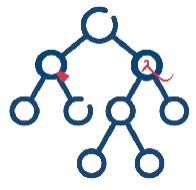
\includegraphics[height=1.0cm]{msca_logo.png}}%
    \end{center}

    \vspace{0.6cm}

    % Main title with Q logos on sides (with clickable links)
    \begin{center}
        \begin{minipage}{0.1\textwidth}
            \centering
            \href{https://quantlet.com}{
\includegraphics[height=1.1cm]{ql_logo.png}}
        \end{minipage}%
        \begin{minipage}{0.78\textwidth}
            \centering
            {\LARGE\bfseries\usebeamercolor[fg]{title}\inserttitle}

            \vspace{0.3cm}

            {\usebeamerfont{subtitle}\usebeamercolor[fg]{title}\insertsubtitle}
        \end{minipage}%
        \begin{minipage}{0.1\textwidth}
            \centering
            \href{https://quantinar.com}{
\includegraphics[height=1.1cm]{qr_logo.png}}
        \end{minipage}
    \end{center}

    \vspace{0.6cm}

    % Authors (left aligned)
    \hspace{0.5cm}{\usebeamerfont{author}\insertauthor}

    \vspace{0.3cm}

    % Institute/Affiliations (left aligned)
    \hspace{0.5cm}\begin{minipage}[t]{0.9\textwidth}
        \raggedright\small\insertinstitute
    \end{minipage}
}

%=============================================================================
% THEOREM ENVIRONMENTS
%=============================================================================
\theoremstyle{definition}
\setbeamertemplate{theorems}[numbered]
\ifdefined\tsalang
\newtheorem{defn}{Definiție}
\newtheorem{thm}{Teoremă}
\newtheorem{prop}{Propoziție}
\newtheorem{rmk}{Observație}
\else
\newtheorem{defn}{Definition}
\newtheorem{thm}{Theorem}
\newtheorem{prop}{Proposition}
\newtheorem{rmk}{Remark}
\fi

%=============================================================================
% CENTRED MINIPAGE (no extra vertical space)
%=============================================================================
\newenvironment{cminipage}[1]{%
    \par\noindent\hfill\begin{minipage}{#1}\ignorespaces
}{%
    \end{minipage}\hfill\null\par
}

%=============================================================================
% CUSTOM COMMANDS
%=============================================================================
\newcommand{\E}{\mathbb{E}}
\newcommand{\Var}{\text{Var}}
\newcommand{\Cov}{\text{Cov}}
\newcommand{\Corr}{\text{Corr}}
\newcommand{\R}{\mathbb{R}}
\newcommand{\N}{\mathbb{N}}
\newcommand{\Z}{\mathbb{Z}}
\newcommand{\B}{\mathbf{B}}
\newcommand{\imark}{\textcolor{MainBlue}{\textbullet}}
\newcommand{\RMSE}{\text{RMSE}}
\newcommand{\MAE}{\text{MAE}}
\newcommand{\MAPE}{\text{MAPE}}

% Boldface vector/matrix commands (VAR, VECM, state space; also used by the older TSA decks)
\newcommand{\bY}{\mathbf{Y}}
\newcommand{\bX}{\mathbf{X}}
\newcommand{\bA}{\mathbf{A}}
\newcommand{\bB}{\mathbf{B}}
\newcommand{\bepsilon}{\boldsymbol{\varepsilon}}
\newcommand{\bSigma}{\boldsymbol{\Sigma}}
\newcommand{\bPhi}{\boldsymbol{\Phi}}
\newcommand{\bGamma}{\boldsymbol{\Gamma}}
\newcommand{\bPi}{\boldsymbol{\Pi}}
\newcommand{\bc}{\mathbf{c}}
\newcommand{\balpha}{\boldsymbol{\alpha}}
\newcommand{\bbeta}{\boldsymbol{\beta}}
\newcommand{\bvarepsilon}{\boldsymbol{\varepsilon}}

% Legacy seminar marks (older TSA seminar decks)
\newcommand{\correct}{\textcolor{Forest}{\checkmark}}
\newcommand{\incorrect}{\textcolor{Crimson}{\texttimes}}
 se definește
%   \newcommand{\coursename}{Time Series Analysis}      (EN)
%   \newcommand{\coursename}{Serii de timp}       (RO)  și  \def\tsalang{ro}
% Fișierele .tex se află în EN/Courses, EN/Seminars, RO/Cursuri, RO/Seminarii (două niveluri sub rădăcină).
% Deck-urile sînt generate de latex/build_chapterN.py / build_seminarN.py (vezi latex/tsa_build.py).

\documentclass[9pt, aspectratio=169, t]{beamer}
\providecommand{\coursename}{Time Series Analysis}

% Ensure content fits on slides
\setbeamersize{text margin left=8mm, text margin right=8mm}
% Smaller institute font (title page)
\setbeamerfont{institute}{size=\footnotesize}

%=============================================================================
% THEME AND STYLE CONFIGURATION
%=============================================================================
\usetheme{default}
% Using default theme for clean header/footer control

% Color Palette (matching Redispatch PDF)
\definecolor{MainBlue}{RGB}{26, 58, 110}
\definecolor{AccentBlue}{RGB}{26, 58, 110}
\definecolor{IDAred}{RGB}{205, 0, 0}
\definecolor{DarkGray}{RGB}{51, 51, 51}
\definecolor{MediumGray}{RGB}{128, 128, 128}
\definecolor{LightGray}{RGB}{248, 248, 248}
\definecolor{VeryLightGray}{RGB}{235, 235, 235}
\definecolor{KeynoteGray}{RGB}{218, 218, 218}
\definecolor{SectionGray}{RGB}{120, 120, 120}
\definecolor{FooterGray}{RGB}{100, 100, 100}
\definecolor{Crimson}{RGB}{220, 53, 69}
\definecolor{Forest}{RGB}{46, 125, 50}
\definecolor{Amber}{RGB}{181, 133, 63}
\definecolor{Orange}{RGB}{230, 126, 34}
\definecolor{Purple}{RGB}{142, 68, 173}

% Gradient background (exact Keynote 315° gradient: white to RGB 218,218,218)
\setbeamertemplate{background}{%
    \begin{tikzpicture}[remember picture, overlay]
        \shade[shading=axis, shading angle=315,
        top color=white, bottom color=KeynoteGray]
        (current page.south west) rectangle (current page.north east);
    \end{tikzpicture}%
}
% Fallback solid color for compatibility
\setbeamercolor{background canvas}{bg=}

\setbeamercolor{palette primary}{bg=MainBlue, fg=white}
\setbeamercolor{palette secondary}{bg=MainBlue!85, fg=white}
\setbeamercolor{palette tertiary}{bg=MainBlue!70, fg=white}
\setbeamercolor{structure}{fg=MainBlue}
\setbeamercolor{title}{fg=IDAred}
\setbeamercolor{frametitle}{fg=IDAred, bg=}
\setbeamercolor{block title}{bg=MainBlue, fg=white}
\setbeamercolor{block body}{bg=VeryLightGray, fg=DarkGray}
\setbeamercolor{block title alerted}{bg=Crimson, fg=white}
\setbeamercolor{block body alerted}{bg=Crimson!8, fg=DarkGray}
\setbeamercolor{block title example}{bg=Forest, fg=white}
\setbeamercolor{block body example}{bg=Forest!8, fg=DarkGray}
\setbeamercolor{item}{fg=MainBlue}

% Footer colors (override Madrid theme blue)
\setbeamercolor{author in head/foot}{fg=FooterGray, bg=}
\setbeamercolor{title in head/foot}{fg=FooterGray, bg=}
\setbeamercolor{date in head/foot}{fg=FooterGray, bg=}
\setbeamercolor{section in head/foot}{fg=FooterGray, bg=}
\setbeamercolor{subsection in head/foot}{fg=FooterGray, bg=}

% Bullet styles (apply everywhere including blocks)
\setbeamertemplate{itemize item}{\color{MainBlue}$\boxdot$}
\setbeamertemplate{itemize subitem}{\color{MainBlue}$\blacktriangleright$}
\setbeamertemplate{itemize subsubitem}{\color{MainBlue}\tiny$\bullet$}
\setbeamertemplate{itemize/enumerate body begin}{\normalsize}
\setbeamertemplate{itemize/enumerate subbody begin}{\normalsize}

% Item spacing - compact style
\setlength{\leftmargini}{10pt}       % Level 1: minimal indent
\setlength{\leftmarginii}{10pt}      % Level 2: minimal additional indent
% Compact list spacing (zero extra space before/after lists in blocks)
\makeatletter
\def\@listi{\leftmargin\leftmargini \topsep 0pt \parsep 0pt \itemsep 0pt}
\def\@listii{\leftmargin\leftmarginii \topsep 0pt \parsep 0pt \itemsep 0pt}
\makeatother

\setbeamertemplate{navigation symbols}{}

%=============================================================================
% CUSTOM HEADLINE
%=============================================================================
\setbeamertemplate{headline}{%
    \vskip10pt%
    \hbox to \paperwidth{%
        \hskip0.5cm%
        {\small\color{FooterGray}\renewcommand{\hyperlink}[2]{##2}\insertsectionhead}%
        \hfill%
        \textcolor{FooterGray}{\small\insertframenumber}%
        \hskip0.5cm%
    }%
    \vskip4pt%
    {\color{FooterGray}\hrule height 0.4pt}%
}

%=============================================================================
% CUSTOM FOOTER
%=============================================================================
\usepackage{fontawesome5}

\setbeamertemplate{footline}{%
    {\color{FooterGray}\hrule height 0.4pt}%
    \vskip4pt%
    \hbox to \paperwidth{%
        \hskip0.5cm%
        \textcolor{FooterGray}{\small\coursename}%
        \hfill%
        \raisebox{-0.1em}{%
            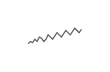
\begin{tikzpicture}[x=0.08em, y=0.08em, line width=0.4pt]
                \draw[FooterGray] (0,3) -- (1,4) -- (2,3.5) -- (3,5) -- (4,4) -- (5,6) -- (6,5.5) -- (7,4) -- (8,5) -- (9,7) -- (10,6) -- (11,5) -- (12,6.5) -- (13,8) -- (14,7) -- (15,6) -- (16,7.5) -- (17,9) -- (18,8) -- (19,7) -- (20,8.5) -- (21,10) -- (22,9) -- (23,8) -- (24,9.5);
            \end{tikzpicture}%
        }%
        \hskip0.5cm%
    }%
    \vskip6pt%
}

%=============================================================================
% PACKAGES
%=============================================================================
\usepackage[utf8]{inputenc}
\DeclareUnicodeCharacter{03B1}{\ensuremath{\alpha}}
\usepackage[T1]{fontenc}
\usepackage{amsmath, amssymb, amsthm}
\usepackage{mathtools}
\usepackage{bm}
\usepackage{tikz}
\usetikzlibrary{arrows.meta, positioning, shapes, calc, decorations.pathreplacing, shadings}
\usepackage{booktabs}
\usepackage{multirow}
\usepackage{array}
\usepackage{graphicx}
\usepackage{animate}
\usepackage{hyperref}
\usepackage{colortbl}
\usepackage{listings}
\lstset{language=Python, basicstyle=\ttfamily\scriptsize, keywordstyle=\color{MainBlue}\bfseries,
  commentstyle=\color{Forest}, stringstyle=\color{Crimson}, breaklines=true,
  frame=none, backgroundcolor=\color{VeryLightGray}, xleftmargin=2mm}
\hypersetup{colorlinks=true, linkcolor=MainBlue, urlcolor=MainBlue}
\graphicspath{{../../logos/}{../../charts/}{../../photos/}}
\usepackage{xcolor}
\hfuzz=2pt  % Suppress tiny overfull warnings (<2pt)
\vfuzz=2pt  % Suppress tiny vertical overfull warnings (<2pt)
% \mathrm in the sans-serif family of the slides (beamer resets \mathrm to the serif family at \begin{document};
% this hook runs after beamer's, so WN, Var, RMSE, ... in formulas match the surrounding text)
% Bold vectors and matrices in the same sans-serif family: \mathbf{A} in sans bold (beamer's own \mathbf came out in
% medium weight), and the bold upright Greek capitals of \boldsymbol / \bm (\bSigma, \bPhi, \boldsymbol{\Theta}) in
% cmss bold: bm.sty fixes its "boldoperators" font when it is loaded (serif cmbx), before beamer switches the
% operators to cmss, so it is reset here.
\AtBeginDocument{%
  \SetMathAlphabet{\mathrm}{normal}{\encodingdefault}{\sfdefault}{\mddefault}{n}%
  \SetMathAlphabet{\mathrm}{bold}{\encodingdefault}{\sfdefault}{bx}{n}%
  \SetMathAlphabet{\mathbf}{normal}{\encodingdefault}{\sfdefault}{bx}{n}%
  \SetMathAlphabet{\mathbf}{bold}{\encodingdefault}{\sfdefault}{bx}{n}%
  \SetSymbolFont{boldoperators}{normal}{OT1}{cmss}{bx}{n}%
  \SetSymbolFont{boldoperators}{bold}{OT1}{cmss}{bx}{n}}

%=============================================================================
% QUANTLET COMMANDS
%   \quantlet{<displayed name>}{<url>}       (generic, compatible with the older TSA decks)
%   \tsaquantlet{Ch_05}{TSA_ch5_garch}       -> https://github.com/danpele/Time-Series-Analysis/tree/main/Quantlets/Ch_05/TSA_ch5_garch
%   \qlurl{<folder>} is defined per chapter by the generator (Quantlets/Ch_NN/<folder>)
%=============================================================================
\newcommand{\tsarepo}{https://github.com/danpele/Time-Series-Analysis}
\newcommand{\tsaqlbase}{https://github.com/danpele/Time-Series-Analysis/tree/main/Quantlets}
\newcommand{\quantlet}[2]{%
    \hfill\href{#2}{%
        \raisebox{-0.15em}{
\includegraphics[height=0.7em]{ql_logo.png}}%
        \textcolor{MainBlue}{\tiny\ #1}%
    }%
}
\newcommand{\tsaquantlet}[2]{\quantlet{\detokenize{#2}}{\tsaqlbase/#1/#2}}

%=============================================================================
% NOTEBOOKS (Google Colab)
%   \colaburl{notebooks/EN/chapter5_seminar_notebook.ipynb} -> the Colab link of a file in the TSA repo
%   \nb: the chapter notebook (each seminar deck redefines it with \renewcommand)
%=============================================================================
\newcommand{\colaburl}[1]{https://colab.research.google.com/github/danpele/Time-Series-Analysis/blob/main/#1}
\newcommand{\nb}{https://colab.research.google.com/github/danpele/Time-Series-Analysis/tree/main/notebooks/EN}
\newcommand{\nbname}{notebooks/EN}

%=============================================================================
% SLIDE HELPERS (used by the generators; the same as in MFM)
%=============================================================================
% local font size for list bodies (the preamble forces \normalsize)
\newcommand{\itemsize}[1]{\setbeamertemplate{itemize/enumerate body begin}{#1}\setbeamertemplate{itemize/enumerate subbody begin}{#1}}
\newcommand{\intitle}[1]{{\hypersetup{urlcolor=white}#1}}   % white links inside coloured title bars
\newcommand{\imgcap}[1]{{\scriptsize #1}\\[0.5mm]}          % caption under a photo
\newcommand{\imgcredit}[2]{{\tiny\color{FooterGray}\href{#1}{#2}}}   % image credit: source URL, author/licence
\newcommand{\aiprompt}[1]{{\ttfamily\color{MainBlue}#1}}     % a prompt to an AI assistant

%=============================================================================
% SEMINARS: student version by default; the instructor wrapper *_solutions.tex sets \solutionstrue
%=============================================================================
\makeatletter\@ifundefined{ifsolutions}{\expandafter\newif\csname ifsolutions\endcsname}{}\makeatother
\newcommand{\solonly}[1]{\ifsolutions #1\fi}
\newcommand{\propsub}{\ifsolutions\else\framesubtitle{\ifdefined\tsalang Rezolvarea se discută la seminar\else Solution discussed in class\fi}\fi}

%=============================================================================
% APPENDIX AND CHAPTER LINKS (latex/appendix_links.py writes the calls; it also re-declares these
% macros before \begin{document}, so the decks compile with or without this preamble block)
%=============================================================================
\providecommand{\tsaapplink}[3]{\hypertarget{#2}{}\hyperlink{#1}{\beamergotobutton{#3}}}
\providecommand{\tsaappback}[2]{\begin{tikzpicture}[remember picture,overlay]\node[anchor=south east] at ([xshift=-3mm,yshift=7mm]current page.south east){\hyperlink{#1}{\beamerreturnbutton{#2}}};\end{tikzpicture}}
\providecommand{\tsachlink}[2]{\href{#1}{#2}}
\providecommand{\tsachlinkt}[2]{\href{#1}{\usebeamercolor[fg]{frametitle}#2}}

%=============================================================================
% QUANTINAR COMMAND: link către un curs Quantinar (subiecte avansate)
%=============================================================================
\newcommand{\quantinar}[2]{%
    \href{#2}{%
        \raisebox{-0.15em}{
\includegraphics[height=0.8em]{qr_logo.png}}%
        \textcolor{MainBlue}{\scriptsize\ #1}%
    }%
}

%=============================================================================
% CUSTOM TITLE PAGE
%=============================================================================
\defbeamertemplate*{title page}{hybrid}[1][]
{
    \vspace{0.2cm}
    % Logos row - top header (with clickable links)
    \begin{center}
        \href{https://www.ase.ro}{
\includegraphics[height=1.0cm]{ase_logo.png}}\hspace{0.3cm}%
        \href{https://theida.net}{
\includegraphics[height=1.0cm]{ida_logo.png}}\hspace{0.3cm}%
        \href{https://blockchain-research-center.com}{
\includegraphics[height=1.0cm]{brc_logo.png}}\hspace{0.3cm}%
        \href{https://www.ai4efin.ase.ro}{
\includegraphics[height=1.0cm]{ai4efin_logo.png}}\hspace{0.3cm}%
        \href{https://ipe.ro/new}{
\includegraphics[height=1.0cm]{acad_logo.png}}\hspace{0.3cm}%
        \href{https://www.digital-finance-msca.com}{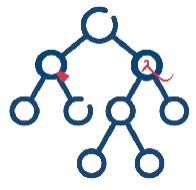
\includegraphics[height=1.0cm]{msca_logo.png}}%
    \end{center}

    \vspace{0.6cm}

    % Main title with Q logos on sides (with clickable links)
    \begin{center}
        \begin{minipage}{0.1\textwidth}
            \centering
            \href{https://quantlet.com}{
\includegraphics[height=1.1cm]{ql_logo.png}}
        \end{minipage}%
        \begin{minipage}{0.78\textwidth}
            \centering
            {\LARGE\bfseries\usebeamercolor[fg]{title}\inserttitle}

            \vspace{0.3cm}

            {\usebeamerfont{subtitle}\usebeamercolor[fg]{title}\insertsubtitle}
        \end{minipage}%
        \begin{minipage}{0.1\textwidth}
            \centering
            \href{https://quantinar.com}{
\includegraphics[height=1.1cm]{qr_logo.png}}
        \end{minipage}
    \end{center}

    \vspace{0.6cm}

    % Authors (left aligned)
    \hspace{0.5cm}{\usebeamerfont{author}\insertauthor}

    \vspace{0.3cm}

    % Institute/Affiliations (left aligned)
    \hspace{0.5cm}\begin{minipage}[t]{0.9\textwidth}
        \raggedright\small\insertinstitute
    \end{minipage}
}

%=============================================================================
% THEOREM ENVIRONMENTS
%=============================================================================
\theoremstyle{definition}
\setbeamertemplate{theorems}[numbered]
\ifdefined\tsalang
\newtheorem{defn}{Definiție}
\newtheorem{thm}{Teoremă}
\newtheorem{prop}{Propoziție}
\newtheorem{rmk}{Observație}
\else
\newtheorem{defn}{Definition}
\newtheorem{thm}{Theorem}
\newtheorem{prop}{Proposition}
\newtheorem{rmk}{Remark}
\fi

%=============================================================================
% CENTRED MINIPAGE (no extra vertical space)
%=============================================================================
\newenvironment{cminipage}[1]{%
    \par\noindent\hfill\begin{minipage}{#1}\ignorespaces
}{%
    \end{minipage}\hfill\null\par
}

%=============================================================================
% CUSTOM COMMANDS
%=============================================================================
\newcommand{\E}{\mathbb{E}}
\newcommand{\Var}{\text{Var}}
\newcommand{\Cov}{\text{Cov}}
\newcommand{\Corr}{\text{Corr}}
\newcommand{\R}{\mathbb{R}}
\newcommand{\N}{\mathbb{N}}
\newcommand{\Z}{\mathbb{Z}}
\newcommand{\B}{\mathbf{B}}
\newcommand{\imark}{\textcolor{MainBlue}{\textbullet}}
\newcommand{\RMSE}{\text{RMSE}}
\newcommand{\MAE}{\text{MAE}}
\newcommand{\MAPE}{\text{MAPE}}

% Boldface vector/matrix commands (VAR, VECM, state space; also used by the older TSA decks)
\newcommand{\bY}{\mathbf{Y}}
\newcommand{\bX}{\mathbf{X}}
\newcommand{\bA}{\mathbf{A}}
\newcommand{\bB}{\mathbf{B}}
\newcommand{\bepsilon}{\boldsymbol{\varepsilon}}
\newcommand{\bSigma}{\boldsymbol{\Sigma}}
\newcommand{\bPhi}{\boldsymbol{\Phi}}
\newcommand{\bGamma}{\boldsymbol{\Gamma}}
\newcommand{\bPi}{\boldsymbol{\Pi}}
\newcommand{\bc}{\mathbf{c}}
\newcommand{\balpha}{\boldsymbol{\alpha}}
\newcommand{\bbeta}{\boldsymbol{\beta}}
\newcommand{\bvarepsilon}{\boldsymbol{\varepsilon}}

% Legacy seminar marks (older TSA seminar decks)
\newcommand{\correct}{\textcolor{Forest}{\checkmark}}
\newcommand{\incorrect}{\textcolor{Crimson}{\texttimes}}
 se definește
%   \newcommand{\coursename}{Time Series Analysis}      (EN)
%   \newcommand{\coursename}{Serii de timp}       (RO)  și  \def\tsalang{ro}
% Fișierele .tex se află în EN/Courses, EN/Seminars, RO/Cursuri, RO/Seminarii (două niveluri sub rădăcină).
% Deck-urile sînt generate de latex/build_chapterN.py / build_seminarN.py (vezi latex/tsa_build.py).

\documentclass[9pt, aspectratio=169, t]{beamer}
\providecommand{\coursename}{Time Series Analysis}

% Ensure content fits on slides
\setbeamersize{text margin left=8mm, text margin right=8mm}
% Smaller institute font (title page)
\setbeamerfont{institute}{size=\footnotesize}

%=============================================================================
% THEME AND STYLE CONFIGURATION
%=============================================================================
\usetheme{default}
% Using default theme for clean header/footer control

% Color Palette (matching Redispatch PDF)
\definecolor{MainBlue}{RGB}{26, 58, 110}
\definecolor{AccentBlue}{RGB}{26, 58, 110}
\definecolor{IDAred}{RGB}{205, 0, 0}
\definecolor{DarkGray}{RGB}{51, 51, 51}
\definecolor{MediumGray}{RGB}{128, 128, 128}
\definecolor{LightGray}{RGB}{248, 248, 248}
\definecolor{VeryLightGray}{RGB}{235, 235, 235}
\definecolor{KeynoteGray}{RGB}{218, 218, 218}
\definecolor{SectionGray}{RGB}{120, 120, 120}
\definecolor{FooterGray}{RGB}{100, 100, 100}
\definecolor{Crimson}{RGB}{220, 53, 69}
\definecolor{Forest}{RGB}{46, 125, 50}
\definecolor{Amber}{RGB}{181, 133, 63}
\definecolor{Orange}{RGB}{230, 126, 34}
\definecolor{Purple}{RGB}{142, 68, 173}

% Gradient background (exact Keynote 315° gradient: white to RGB 218,218,218)
\setbeamertemplate{background}{%
    \begin{tikzpicture}[remember picture, overlay]
        \shade[shading=axis, shading angle=315,
        top color=white, bottom color=KeynoteGray]
        (current page.south west) rectangle (current page.north east);
    \end{tikzpicture}%
}
% Fallback solid color for compatibility
\setbeamercolor{background canvas}{bg=}

\setbeamercolor{palette primary}{bg=MainBlue, fg=white}
\setbeamercolor{palette secondary}{bg=MainBlue!85, fg=white}
\setbeamercolor{palette tertiary}{bg=MainBlue!70, fg=white}
\setbeamercolor{structure}{fg=MainBlue}
\setbeamercolor{title}{fg=IDAred}
\setbeamercolor{frametitle}{fg=IDAred, bg=}
\setbeamercolor{block title}{bg=MainBlue, fg=white}
\setbeamercolor{block body}{bg=VeryLightGray, fg=DarkGray}
\setbeamercolor{block title alerted}{bg=Crimson, fg=white}
\setbeamercolor{block body alerted}{bg=Crimson!8, fg=DarkGray}
\setbeamercolor{block title example}{bg=Forest, fg=white}
\setbeamercolor{block body example}{bg=Forest!8, fg=DarkGray}
\setbeamercolor{item}{fg=MainBlue}

% Footer colors (override Madrid theme blue)
\setbeamercolor{author in head/foot}{fg=FooterGray, bg=}
\setbeamercolor{title in head/foot}{fg=FooterGray, bg=}
\setbeamercolor{date in head/foot}{fg=FooterGray, bg=}
\setbeamercolor{section in head/foot}{fg=FooterGray, bg=}
\setbeamercolor{subsection in head/foot}{fg=FooterGray, bg=}

% Bullet styles (apply everywhere including blocks)
\setbeamertemplate{itemize item}{\color{MainBlue}$\boxdot$}
\setbeamertemplate{itemize subitem}{\color{MainBlue}$\blacktriangleright$}
\setbeamertemplate{itemize subsubitem}{\color{MainBlue}\tiny$\bullet$}
\setbeamertemplate{itemize/enumerate body begin}{\normalsize}
\setbeamertemplate{itemize/enumerate subbody begin}{\normalsize}

% Item spacing - compact style
\setlength{\leftmargini}{10pt}       % Level 1: minimal indent
\setlength{\leftmarginii}{10pt}      % Level 2: minimal additional indent
% Compact list spacing (zero extra space before/after lists in blocks)
\makeatletter
\def\@listi{\leftmargin\leftmargini \topsep 0pt \parsep 0pt \itemsep 0pt}
\def\@listii{\leftmargin\leftmarginii \topsep 0pt \parsep 0pt \itemsep 0pt}
\makeatother

\setbeamertemplate{navigation symbols}{}

%=============================================================================
% CUSTOM HEADLINE
%=============================================================================
\setbeamertemplate{headline}{%
    \vskip10pt%
    \hbox to \paperwidth{%
        \hskip0.5cm%
        {\small\color{FooterGray}\renewcommand{\hyperlink}[2]{##2}\insertsectionhead}%
        \hfill%
        \textcolor{FooterGray}{\small\insertframenumber}%
        \hskip0.5cm%
    }%
    \vskip4pt%
    {\color{FooterGray}\hrule height 0.4pt}%
}

%=============================================================================
% CUSTOM FOOTER
%=============================================================================
\usepackage{fontawesome5}

\setbeamertemplate{footline}{%
    {\color{FooterGray}\hrule height 0.4pt}%
    \vskip4pt%
    \hbox to \paperwidth{%
        \hskip0.5cm%
        \textcolor{FooterGray}{\small\coursename}%
        \hfill%
        \raisebox{-0.1em}{%
            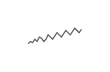
\begin{tikzpicture}[x=0.08em, y=0.08em, line width=0.4pt]
                \draw[FooterGray] (0,3) -- (1,4) -- (2,3.5) -- (3,5) -- (4,4) -- (5,6) -- (6,5.5) -- (7,4) -- (8,5) -- (9,7) -- (10,6) -- (11,5) -- (12,6.5) -- (13,8) -- (14,7) -- (15,6) -- (16,7.5) -- (17,9) -- (18,8) -- (19,7) -- (20,8.5) -- (21,10) -- (22,9) -- (23,8) -- (24,9.5);
            \end{tikzpicture}%
        }%
        \hskip0.5cm%
    }%
    \vskip6pt%
}

%=============================================================================
% PACKAGES
%=============================================================================
\usepackage[utf8]{inputenc}
\DeclareUnicodeCharacter{03B1}{\ensuremath{\alpha}}
\usepackage[T1]{fontenc}
\usepackage{amsmath, amssymb, amsthm}
\usepackage{mathtools}
\usepackage{bm}
\usepackage{tikz}
\usetikzlibrary{arrows.meta, positioning, shapes, calc, decorations.pathreplacing, shadings}
\usepackage{booktabs}
\usepackage{multirow}
\usepackage{array}
\usepackage{graphicx}
\usepackage{animate}
\usepackage{hyperref}
\usepackage{colortbl}
\usepackage{listings}
\lstset{language=Python, basicstyle=\ttfamily\scriptsize, keywordstyle=\color{MainBlue}\bfseries,
  commentstyle=\color{Forest}, stringstyle=\color{Crimson}, breaklines=true,
  frame=none, backgroundcolor=\color{VeryLightGray}, xleftmargin=2mm}
\hypersetup{colorlinks=true, linkcolor=MainBlue, urlcolor=MainBlue}
\graphicspath{{../../logos/}{../../charts/}{../../photos/}}
\usepackage{xcolor}
\hfuzz=2pt  % Suppress tiny overfull warnings (<2pt)
\vfuzz=2pt  % Suppress tiny vertical overfull warnings (<2pt)
% \mathrm in the sans-serif family of the slides (beamer resets \mathrm to the serif family at \begin{document};
% this hook runs after beamer's, so WN, Var, RMSE, ... in formulas match the surrounding text)
% Bold vectors and matrices in the same sans-serif family: \mathbf{A} in sans bold (beamer's own \mathbf came out in
% medium weight), and the bold upright Greek capitals of \boldsymbol / \bm (\bSigma, \bPhi, \boldsymbol{\Theta}) in
% cmss bold: bm.sty fixes its "boldoperators" font when it is loaded (serif cmbx), before beamer switches the
% operators to cmss, so it is reset here.
\AtBeginDocument{%
  \SetMathAlphabet{\mathrm}{normal}{\encodingdefault}{\sfdefault}{\mddefault}{n}%
  \SetMathAlphabet{\mathrm}{bold}{\encodingdefault}{\sfdefault}{bx}{n}%
  \SetMathAlphabet{\mathbf}{normal}{\encodingdefault}{\sfdefault}{bx}{n}%
  \SetMathAlphabet{\mathbf}{bold}{\encodingdefault}{\sfdefault}{bx}{n}%
  \SetSymbolFont{boldoperators}{normal}{OT1}{cmss}{bx}{n}%
  \SetSymbolFont{boldoperators}{bold}{OT1}{cmss}{bx}{n}}

%=============================================================================
% QUANTLET COMMANDS
%   \quantlet{<displayed name>}{<url>}       (generic, compatible with the older TSA decks)
%   \tsaquantlet{Ch_05}{TSA_ch5_garch}       -> https://github.com/danpele/Time-Series-Analysis/tree/main/Quantlets/Ch_05/TSA_ch5_garch
%   \qlurl{<folder>} is defined per chapter by the generator (Quantlets/Ch_NN/<folder>)
%=============================================================================
\newcommand{\tsarepo}{https://github.com/danpele/Time-Series-Analysis}
\newcommand{\tsaqlbase}{https://github.com/danpele/Time-Series-Analysis/tree/main/Quantlets}
\newcommand{\quantlet}[2]{%
    \hfill\href{#2}{%
        \raisebox{-0.15em}{
\includegraphics[height=0.7em]{ql_logo.png}}%
        \textcolor{MainBlue}{\tiny\ #1}%
    }%
}
\newcommand{\tsaquantlet}[2]{\quantlet{\detokenize{#2}}{\tsaqlbase/#1/#2}}

%=============================================================================
% NOTEBOOKS (Google Colab)
%   \colaburl{notebooks/EN/chapter5_seminar_notebook.ipynb} -> the Colab link of a file in the TSA repo
%   \nb: the chapter notebook (each seminar deck redefines it with \renewcommand)
%=============================================================================
\newcommand{\colaburl}[1]{https://colab.research.google.com/github/danpele/Time-Series-Analysis/blob/main/#1}
\newcommand{\nb}{https://colab.research.google.com/github/danpele/Time-Series-Analysis/tree/main/notebooks/EN}
\newcommand{\nbname}{notebooks/EN}

%=============================================================================
% SLIDE HELPERS (used by the generators; the same as in MFM)
%=============================================================================
% local font size for list bodies (the preamble forces \normalsize)
\newcommand{\itemsize}[1]{\setbeamertemplate{itemize/enumerate body begin}{#1}\setbeamertemplate{itemize/enumerate subbody begin}{#1}}
\newcommand{\intitle}[1]{{\hypersetup{urlcolor=white}#1}}   % white links inside coloured title bars
\newcommand{\imgcap}[1]{{\scriptsize #1}\\[0.5mm]}          % caption under a photo
\newcommand{\imgcredit}[2]{{\tiny\color{FooterGray}\href{#1}{#2}}}   % image credit: source URL, author/licence
\newcommand{\aiprompt}[1]{{\ttfamily\color{MainBlue}#1}}     % a prompt to an AI assistant

%=============================================================================
% SEMINARS: student version by default; the instructor wrapper *_solutions.tex sets \solutionstrue
%=============================================================================
\makeatletter\@ifundefined{ifsolutions}{\expandafter\newif\csname ifsolutions\endcsname}{}\makeatother
\newcommand{\solonly}[1]{\ifsolutions #1\fi}
\newcommand{\propsub}{\ifsolutions\else\framesubtitle{\ifdefined\tsalang Rezolvarea se discută la seminar\else Solution discussed in class\fi}\fi}

%=============================================================================
% APPENDIX AND CHAPTER LINKS (latex/appendix_links.py writes the calls; it also re-declares these
% macros before \begin{document}, so the decks compile with or without this preamble block)
%=============================================================================
\providecommand{\tsaapplink}[3]{\hypertarget{#2}{}\hyperlink{#1}{\beamergotobutton{#3}}}
\providecommand{\tsaappback}[2]{\begin{tikzpicture}[remember picture,overlay]\node[anchor=south east] at ([xshift=-3mm,yshift=7mm]current page.south east){\hyperlink{#1}{\beamerreturnbutton{#2}}};\end{tikzpicture}}
\providecommand{\tsachlink}[2]{\href{#1}{#2}}
\providecommand{\tsachlinkt}[2]{\href{#1}{\usebeamercolor[fg]{frametitle}#2}}

%=============================================================================
% QUANTINAR COMMAND: link către un curs Quantinar (subiecte avansate)
%=============================================================================
\newcommand{\quantinar}[2]{%
    \href{#2}{%
        \raisebox{-0.15em}{
\includegraphics[height=0.8em]{qr_logo.png}}%
        \textcolor{MainBlue}{\scriptsize\ #1}%
    }%
}

%=============================================================================
% CUSTOM TITLE PAGE
%=============================================================================
\defbeamertemplate*{title page}{hybrid}[1][]
{
    \vspace{0.2cm}
    % Logos row - top header (with clickable links)
    \begin{center}
        \href{https://www.ase.ro}{
\includegraphics[height=1.0cm]{ase_logo.png}}\hspace{0.3cm}%
        \href{https://theida.net}{
\includegraphics[height=1.0cm]{ida_logo.png}}\hspace{0.3cm}%
        \href{https://blockchain-research-center.com}{
\includegraphics[height=1.0cm]{brc_logo.png}}\hspace{0.3cm}%
        \href{https://www.ai4efin.ase.ro}{
\includegraphics[height=1.0cm]{ai4efin_logo.png}}\hspace{0.3cm}%
        \href{https://ipe.ro/new}{
\includegraphics[height=1.0cm]{acad_logo.png}}\hspace{0.3cm}%
        \href{https://www.digital-finance-msca.com}{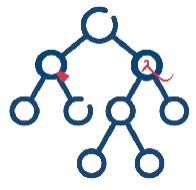
\includegraphics[height=1.0cm]{msca_logo.png}}%
    \end{center}

    \vspace{0.6cm}

    % Main title with Q logos on sides (with clickable links)
    \begin{center}
        \begin{minipage}{0.1\textwidth}
            \centering
            \href{https://quantlet.com}{
\includegraphics[height=1.1cm]{ql_logo.png}}
        \end{minipage}%
        \begin{minipage}{0.78\textwidth}
            \centering
            {\LARGE\bfseries\usebeamercolor[fg]{title}\inserttitle}

            \vspace{0.3cm}

            {\usebeamerfont{subtitle}\usebeamercolor[fg]{title}\insertsubtitle}
        \end{minipage}%
        \begin{minipage}{0.1\textwidth}
            \centering
            \href{https://quantinar.com}{
\includegraphics[height=1.1cm]{qr_logo.png}}
        \end{minipage}
    \end{center}

    \vspace{0.6cm}

    % Authors (left aligned)
    \hspace{0.5cm}{\usebeamerfont{author}\insertauthor}

    \vspace{0.3cm}

    % Institute/Affiliations (left aligned)
    \hspace{0.5cm}\begin{minipage}[t]{0.9\textwidth}
        \raggedright\small\insertinstitute
    \end{minipage}
}

%=============================================================================
% THEOREM ENVIRONMENTS
%=============================================================================
\theoremstyle{definition}
\setbeamertemplate{theorems}[numbered]
\ifdefined\tsalang
\newtheorem{defn}{Definiție}
\newtheorem{thm}{Teoremă}
\newtheorem{prop}{Propoziție}
\newtheorem{rmk}{Observație}
\else
\newtheorem{defn}{Definition}
\newtheorem{thm}{Theorem}
\newtheorem{prop}{Proposition}
\newtheorem{rmk}{Remark}
\fi

%=============================================================================
% CENTRED MINIPAGE (no extra vertical space)
%=============================================================================
\newenvironment{cminipage}[1]{%
    \par\noindent\hfill\begin{minipage}{#1}\ignorespaces
}{%
    \end{minipage}\hfill\null\par
}

%=============================================================================
% CUSTOM COMMANDS
%=============================================================================
\newcommand{\E}{\mathbb{E}}
\newcommand{\Var}{\text{Var}}
\newcommand{\Cov}{\text{Cov}}
\newcommand{\Corr}{\text{Corr}}
\newcommand{\R}{\mathbb{R}}
\newcommand{\N}{\mathbb{N}}
\newcommand{\Z}{\mathbb{Z}}
\newcommand{\B}{\mathbf{B}}
\newcommand{\imark}{\textcolor{MainBlue}{\textbullet}}
\newcommand{\RMSE}{\text{RMSE}}
\newcommand{\MAE}{\text{MAE}}
\newcommand{\MAPE}{\text{MAPE}}

% Boldface vector/matrix commands (VAR, VECM, state space; also used by the older TSA decks)
\newcommand{\bY}{\mathbf{Y}}
\newcommand{\bX}{\mathbf{X}}
\newcommand{\bA}{\mathbf{A}}
\newcommand{\bB}{\mathbf{B}}
\newcommand{\bepsilon}{\boldsymbol{\varepsilon}}
\newcommand{\bSigma}{\boldsymbol{\Sigma}}
\newcommand{\bPhi}{\boldsymbol{\Phi}}
\newcommand{\bGamma}{\boldsymbol{\Gamma}}
\newcommand{\bPi}{\boldsymbol{\Pi}}
\newcommand{\bc}{\mathbf{c}}
\newcommand{\balpha}{\boldsymbol{\alpha}}
\newcommand{\bbeta}{\boldsymbol{\beta}}
\newcommand{\bvarepsilon}{\boldsymbol{\varepsilon}}

% Legacy seminar marks (older TSA seminar decks)
\newcommand{\correct}{\textcolor{Forest}{\checkmark}}
\newcommand{\incorrect}{\textcolor{Crimson}{\texttimes}}


\newcommand{\qlurl}[1]{https://github.com/danpele/Time-Series-Analysis/tree/main/Quantlets/Ch_12/#1}

% Clickable citations (DOIs verified via Crossref)
\newcommand{\refHP}{\href{https://doi.org/10.1007/978-3-031-13584-2}{Huang and Petukhina (2022)}}
\newcommand{\refSS}{\href{https://doi.org/10.1007/978-3-319-52452-8}{Shumway and Stoffer (2017)}}
\newcommand{\refBDtm}{\href{https://doi.org/10.1007/978-1-4419-0320-4}{Brockwell and Davis (1991)}}
\newcommand{\refHamTS}{\href{https://doi.org/10.1515/9780691218632}{Hamilton (1994)}}
\newcommand{\refSchuster}{\href{https://doi.org/10.1029/TM003i001p00013}{Schuster (1898)}}
\newcommand{\refYule}{\href{https://doi.org/10.1098/rsta.1927.0007}{Yule (1927)}}
\newcommand{\refFisher}{\href{https://doi.org/10.1098/rspa.1929.0151}{Fisher (1929)}}
\newcommand{\refBartlett}{\href{https://doi.org/10.1093/biomet/37.1-2.1}{Bartlett (1950)}}
\newcommand{\refBT}{\href{https://doi.org/10.1002/j.1538-7305.1958.tb03874.x}{Blackman and Tukey (1958)}}
\newcommand{\refCT}{\href{https://doi.org/10.1090/S0025-5718-1965-0178586-1}{Cooley and Tukey (1965)}}
\newcommand{\refGranger}{\href{https://doi.org/10.2307/1909859}{Granger (1966)}}
\newcommand{\refWelch}{\href{https://doi.org/10.1109/TAU.1967.1161901}{Welch (1967)}}
\newcommand{\refGPH}{\href{https://doi.org/10.1111/j.1467-9892.1983.tb00371.x}{Geweke and Porter-Hudak (1983)}}
\newcommand{\refHPf}{\href{https://doi.org/10.2307/2953682}{Hodrick and Prescott (1997)}}
\newcommand{\refTC}{\href{https://doi.org/10.1175/1520-0477(1998)079<0061:APGTWA>2.0.CO;2}{Torrence and Compo (1998)}}
\newcommand{\refBK}{\href{https://doi.org/10.1162/003465399558454}{Baxter and King (1999)}}
\newcommand{\refHamHP}{\href{https://doi.org/10.1162/rest_a_00706}{Hamilton (2018)}}

\title[Time Series Analysis]{Time Series Analysis}
\subtitle{Chapter 12: Spectral analysis}
\author[D.T. Pele]{Daniel Traian PELE}
\institute{Bucharest University of Economic Studies\\
IDA Institute Digital Assets\\
Blockchain Research Center\\
AI4EFin Artificial Intelligence for Energy Finance\\
Romanian Academy, Institute for Economic Forecasting\\
MSCA Digital Finance}
\date{}

%=============================================================================
\providecommand{\tsaapplink}[3]{\hypertarget{#2}{}\hyperlink{#1}{\beamergotobutton{#3}}}  % APPLINKS-MACROS
\providecommand{\tsaappback}[2]{\begin{tikzpicture}[remember picture,overlay]\node[anchor=south east] at ([xshift=-3mm,yshift=7mm]current page.south east){\hyperlink{#1}{\beamerreturnbutton{#2}}};\end{tikzpicture}}  % APPLINKS-MACROS
\providecommand{\tsachlink}[2]{\href{#1}{#2}}  % APPLINKS-MACROS
\providecommand{\tsachlinkt}[2]{\href{#1}{\usebeamercolor[fg]{frametitle}#2}}  % APPLINKS-MACROS
\begin{document}
%=============================================================================

{
\setbeamertemplate{headline}{}
\setbeamertemplate{footline}{}
\begin{frame}[noframenumbering]
    \titlepage
\end{frame}
}
% BEGIN-ACRONYMS (generat de latex/acronyms.py; nu editati manual)
\begin{frame}{Acronyms used in this material}
\setbeamertemplate{itemize/enumerate body begin}{\tiny}
\begin{columns}[T]
\begin{column}{0.49\textwidth}
\begin{itemize}\setlength{\itemsep}{0pt}
    \item \textbf{ACF}: Autocorrelation Function
    \item \textbf{AI}: Artificial Intelligence
    \item \textbf{AR}: AutoRegressive (model); in event studies: Abnormal Return
    \item \textbf{ARFIMA}: AutoRegressive Fractionally Integrated Moving Average (model)
    \item \textbf{ARMA}: AutoRegressive Moving Average (model)
    \item \textbf{CWT}: Continuous Wavelet Transform
    \item \textbf{DFT}: Discrete Fourier Transform
    \item \textbf{ENTSO-E}: European Network of Transmission System Operators for Electricity
    \item \textbf{EODHD}: EOD Historical Data (market-data provider)
    \item \textbf{EU}: European Union
    \item \textbf{FFT}: Fast Fourier Transform
    \item \textbf{FRED}: Federal Reserve Economic Data
    \item \textbf{GDP}: Gross Domestic Product
\end{itemize}
\end{column}
\begin{column}{0.49\textwidth}
\begin{itemize}\setlength{\itemsep}{0pt}
    \item \textbf{GDPC1}: Real Gross Domestic Product, chained dollars (FRED series code)
    \item \textbf{GPH}: Geweke–Porter-Hudak (estimator)
    \item \textbf{HP}: Hodrick–Prescott (filter)
    \item \textbf{INDPRO}: Industrial Production Index (FRED series code)
    \item \textbf{LPPL}: Log-Periodic Power Law
    \item \textbf{MA}: Moving Average
    \item \textbf{MW}: Megawatt
    \item \textbf{OLS}: Ordinary Least Squares
    \item \textbf{SILSO}: Sunspot Index and Long-term Solar Observations
    \item \textbf{STFT}: Short-Time Fourier Transform
    \item \textbf{UNRATE}: Unemployment Rate (FRED series code)
    \item \textbf{US}: United States
    \item \textbf{UTC}: Coordinated Universal Time (Temps Universel Coordonné)
\end{itemize}
\end{column}
\end{columns}
\end{frame}
% END-ACRONYMS

\begin{frame}{The chapter's question and route}
\itemsize{\small}
\begin{itemize}
    \item \textbf{Question}: which cycles does a series contain, and how much of its variance does each cycle explain?
    \begin{itemize}
        \item examples: the 11-year sunspot cycle, the business cycle, the daily and weekly rhythm of electricity demand
    \end{itemize}
    \item \textbf{Route} of the chapter
    \begin{itemize}
        \item cycles, frequencies and the discrete Fourier transform
        \item the spectral density of white noise and of ARMA models
        \item the periodogram, its weaknesses, and how to smooth it
        \item cycles in data; long memory; filters; two series; wavelets as a pointer
    \end{itemize}
    \item Self-study chapter: worked examples, interpretation slides and a recap after each section; self-assessment with answers at the end
\end{itemize}
\end{frame}

\begin{frame}{Learning outcomes}
\itemsize{\small}
\begin{itemize}
    \item Convert between frequency, period and angular frequency, and find the Fourier frequencies of a sample
    \item Compute the spectral density of white noise, AR(1), MA(1) and AR(2) models and read its shape
    \item Compute a periodogram by hand for a short series and explain why the raw periodogram is not consistent
    \item Smooth the periodogram (Daniell, Bartlett, Welch), taper the data and build chi-square confidence bands
    \item Identify cycles in sunspots, GDP and electricity load; read coherence and phase between two series
\end{itemize}
\end{frame}

\begin{frame}{Reading and tools}
\itemsize{\small}
\begin{itemize}
    \item Main reference for this chapter: \refSS, \tsachlink{https://danpele.github.io/Time-Series-Analysis/EN/Courses/chapter4_seasonality_forecasting.pdf}{Chapter 4} (spectral analysis and filtering)
    \begin{itemize}
        \item theory: \refBDtm, \tsachlink{https://danpele.github.io/Time-Series-Analysis/EN/Courses/chapter4_seasonality_forecasting.pdf}{Chapters 4} and \tsachlink{https://danpele.github.io/Time-Series-Analysis/EN/Courses/chapter10_state_space_kalman_markov_switching.pdf}{10}; \refHamTS, \tsachlink{https://danpele.github.io/Time-Series-Analysis/EN/Courses/chapter6_var_models_granger_causality.pdf}{Chapter 6}; applications in Python: \refHP
        \item \refSS\ measure frequency in cycles per observation; \tsachlink{https://danpele.github.io/Time-Series-Analysis/EN/Courses/chapter8_long_memory_arfima.pdf}{Chapter 8} used the angular frequency $\lambda = 2\pi\nu$
    \end{itemize}
    \item Python Quantlets of this chapter: \href{https://github.com/danpele/Time-Series-Analysis/tree/main/Quantlets/Ch_12}{Quantlets/Ch\_12}
    \begin{itemize}
        \item the periodogram, the Daniell smoother and the Morlet wavelet are written out in \texttt{numpy}; Welch and coherence come from \texttt{scipy.signal}
    \end{itemize}
    \item Lecture notebook: \href{\colaburl{notebooks/EN/chapter12_lecture_notebook.ipynb}}{open in Google Colab}
    \item Video course: \quantinar{Applied Time Series Analysis with Python}{https://quantinar.com/course/137/applied-time-series-analysis-with-python}
\end{itemize}
\end{frame}


%=============================================================================
\section{Cycles and frequencies}
%=============================================================================

\begin{frame}{Joseph Fourier and the idea of the chapter}
\itemsize{\small}
\begin{columns}[T]
\begin{column}{0.36\textwidth}
\centering
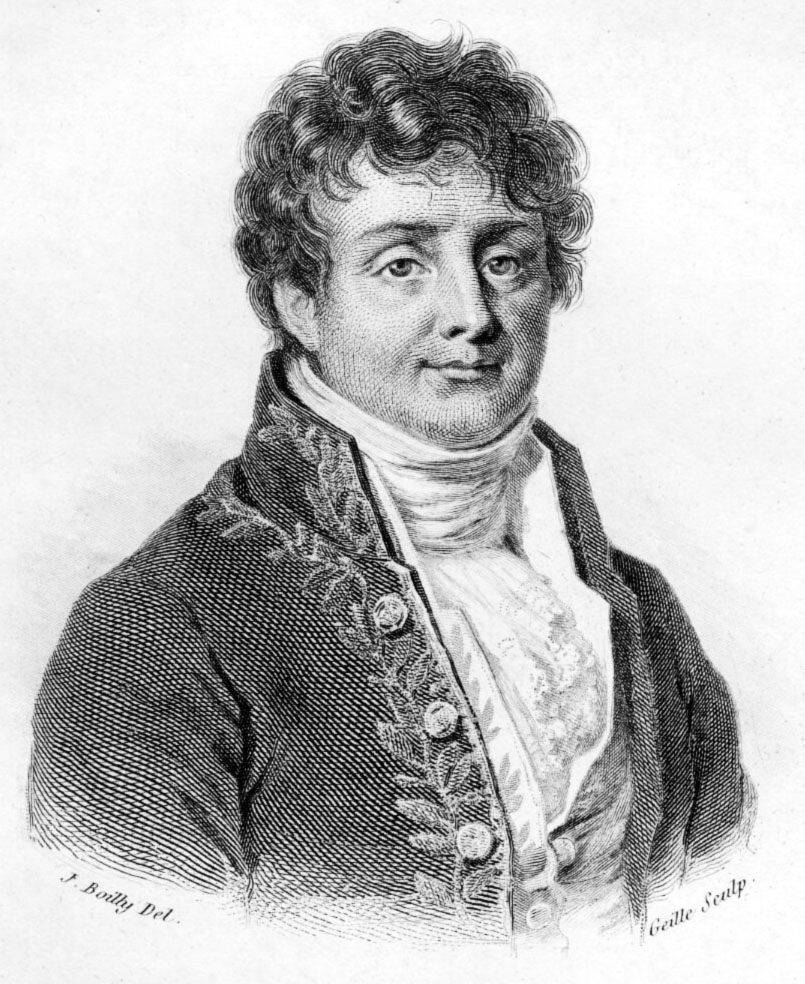
\includegraphics[height=0.5\textheight]{ch12_joseph_fourier.jpg}\\[1mm]
\imgcap{J. B. J. Fourier (1768--1830)}
\imgcredit{https://commons.wikimedia.org/wiki/File:Joseph_Fourier.jpg}{Engraving: A. F. B. Geille, after J.-L. Boilly (1839--1840); public domain; Wikimedia Commons}
\end{column}
\begin{column}{0.62\textwidth}
\begin{itemize}
    \item Fourier (1807, heat conduction): a function can be written as a sum of sines and cosines
    \begin{itemize}
        \item each term is a pure cycle with its own frequency and amplitude
    \end{itemize}
    \item Applied to a time series: how much variance sits at each frequency?
    \begin{itemize}
        \item the \textbf{time domain} (\tsachlink{https://danpele.github.io/Time-Series-Analysis/EN/Courses/chapter1_stochastic_processes_stationarity.pdf}{Chapters 1}--\tsachlink{https://danpele.github.io/Time-Series-Analysis/EN/Courses/chapter8_long_memory_arfima.pdf}{8}) describes the series through its autocorrelations
        \item the \textbf{frequency domain} describes the same information through the spectrum
    \end{itemize}
    \item The two views are equivalent; the spectrum makes cycles visible at a glance
\end{itemize}
\end{column}
\end{columns}
\end{frame}

\begin{frame}{A cycle: amplitude, frequency, phase}
\itemsize{\small}
\begin{itemize}
    \item A pure cycle: $x_t = A\cos(2\pi\nu t + \varphi)$, $t = 1, 2, \ldots$
    \begin{itemize}
        \item $A$: \textbf{amplitude} (height of the wave); $\varphi$: \textbf{phase} (where the wave starts)
        \item $\nu$: \textbf{frequency}, in cycles per observation; the \textbf{period} $1/\nu$ is the number of observations per cycle
        \item angular frequency $\omega = 2\pi\nu$, in radians per observation
    \end{itemize}
    \item Example: monthly data with an annual cycle: $\nu = 1/12$ cycles per month, period 12 months
    \begin{itemize}
        \item hourly data with a daily cycle: $\nu = 1/24$; quarterly data with a 6-year cycle: $\nu = 1/24$ as well
    \end{itemize}
    \item Equivalent form: $A\cos(2\pi\nu t + \varphi) = a\cos(2\pi\nu t) + b\sin(2\pi\nu t)$
    \begin{itemize}
        \item with $a = A\cos\varphi$, $b = -A\sin\varphi$ and $A^2 = a^2 + b^2$: linear in $a$ and $b$, so it can be fitted by OLS
    \end{itemize}
    \item The highest frequency visible in discrete data is $\nu = 1/2$ (one cycle every two observations): the \textbf{Nyquist frequency}
\end{itemize}
\end{frame}

\begin{frame}{Two cycles plus noise}
\itemsize{\footnotesize}
\begin{center}
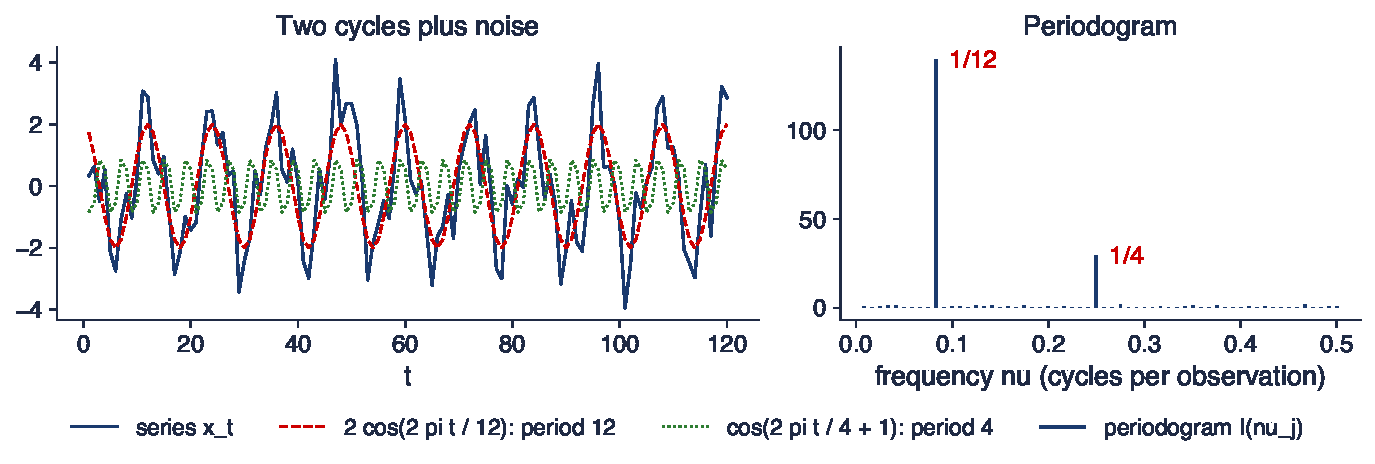
\includegraphics[width=0.97\textwidth,height=0.62\textheight,keepaspectratio]{tsa_ch12_fourier.pdf}
\end{center}
\vspace{-0.25cm}
\begin{itemize}
    \item Simulated series, $T = 120$: $x_t = 2\cos(2\pi t/12) + \cos(2\pi t/4 + 1) + \varepsilon_t$, $\varepsilon_t \sim N(0, 0.49)$ (Normal white noise with variance 0.49); right: its periodogram (defined in Section 3)
\end{itemize}
\quantlet{TSA\_ch12\_fourier}{\qlurl{TSA_ch12_fourier}}
\end{frame}

\begin{frame}{Interpreting two cycles plus noise}
\itemsize{\small}
\begin{itemize}
    \item In the time domain the two cycles are hard to separate by eye
    \begin{itemize}
        \item in the frequency domain they are two isolated spikes, at $\nu = 1/12$ and $\nu = 1/4$
    \end{itemize}
    \item Height of the spikes: 139.7 and 29.6; theory for a cycle of amplitude $A$ at a Fourier frequency: $A^2T/4$, i.e.\ 120 and 30
    \begin{itemize}
        \item the spike grows with the squared amplitude: the larger cycle dominates
    \end{itemize}
    \item The two spikes hold 85\% of the total power; the noise spreads the rest evenly over all frequencies
\end{itemize}
\end{frame}

\begin{frame}{Fourier frequencies and the discrete Fourier transform (1/2)}
\itemsize{\small}
\begin{itemize}
    \item For a sample $x_1, \ldots, x_T$, the \textbf{Fourier frequencies} are $\nu_j = j/T$, $j = 0, 1, \ldots, \lfloor T/2 \rfloor$
    \begin{itemize}
        \item cycles that fit an integer number of times ($j$ times) in the sample; $\lfloor T/2 \rfloor$: the integer part of $T/2$
    \end{itemize}
    \item The \textbf{discrete Fourier transform} (DFT) measures how strongly the series moves with a cycle of frequency $\nu_j$
    \begin{itemize}
        \item $d(\nu_j) = T^{-1/2}\sum_{t=1}^{T} x_t\, e^{-2\pi i \nu_j t}$
        \item $i$: the imaginary unit, $i^2 = -1$; $e^{-i\theta} = \cos\theta - i\sin\theta$ (Euler's formula)
        \item so the DFT correlates the series with a cosine (real part) and a sine (imaginary part) of frequency $\nu_j$
    \end{itemize}
\end{itemize}
\end{frame}

\begin{frame}{Fourier frequencies and the discrete Fourier transform (2/2)}
\itemsize{\small}
\begin{itemize}
    \item The $T$ values $d(\nu_j)$ contain exactly the same information as the $T$ data points
    \begin{itemize}
        \item the data can be recovered from them by the inverse transform
    \end{itemize}
    \item \textbf{Parseval}
    \begin{itemize}
        \item the sum of squared deviations equals the sum of the squared moduli of the DFT
        \item $\sum_{t=1}^{T}(x_t - \bar x)^2 = \sum_{j=1}^{T-1}|d(\nu_j)|^2$
        \item $\bar x$: the sample mean; $|d|^2 = (\mathrm{Re}\,d)^2 + (\mathrm{Im}\,d)^2$: the squared modulus of a complex number
        \item reading: the variance of the series is split over the frequencies
    \end{itemize}
    \item The \textbf{fast Fourier transform} (FFT) of \refCT\ computes all $d(\nu_j)$ quickly
    \begin{itemize}
        \item $O(T\log T)$ operations instead of $O(T^2)$: the number of operations grows like $T\log T$ instead of $T^2$
    \end{itemize}
\end{itemize}
\end{frame}

\begin{frame}{Worked example: the DFT of four numbers}
\itemsize{\small}
\begin{itemize}
    \item Data: $x = (4, 2, 0, 2)$, $T = 4$; mean $\bar x = 2$, deviations $y = (2, 0, -2, 0)$
    \begin{itemize}
        \item Fourier frequencies: $\nu_1 = 1/4$ (period 4) and $\nu_2 = 1/2$ (period 2)
    \end{itemize}
    \item At $\nu = 1/4$: $e^{-2\pi i t/4} = e^{-i\pi t/2}$ equals $-i$ for $t = 1$ and $i$ for $t = 3$
    \begin{itemize}
        \item $\sum_t y_t e^{-i\pi t/2} = 2(-i) + (-2)(i) = -4i$, so $d(1/4) = -4i/\sqrt{4} = -2i$ and $|d(1/4)|^2 = 4$
    \end{itemize}
    \item At $\nu = 1/2$: $e^{-i\pi t} = (-1)^t$, so $\sum_t y_t(-1)^t = -2 + 2 = 0$ and $|d(1/2)|^2 = 0$
    \begin{itemize}
        \item by symmetry $|d(3/4)|^2 = |d(1/4)|^2 = 4$
    \end{itemize}
    \item Parseval: $4 + 0 + 4 = 8 = 2^2 + 0^2 + (-2)^2 + 0^2$; the whole variance ($8/4 = 2$) sits at period 4
    \item Check in Python: \texttt{abs(np.fft.fft([2, 0, -2, 0]))**2 / 4} gives $(0, 4, 0, 4)$
\end{itemize}
\end{frame}

\begin{frame}{Aliasing}
\itemsize{\footnotesize}
\begin{center}
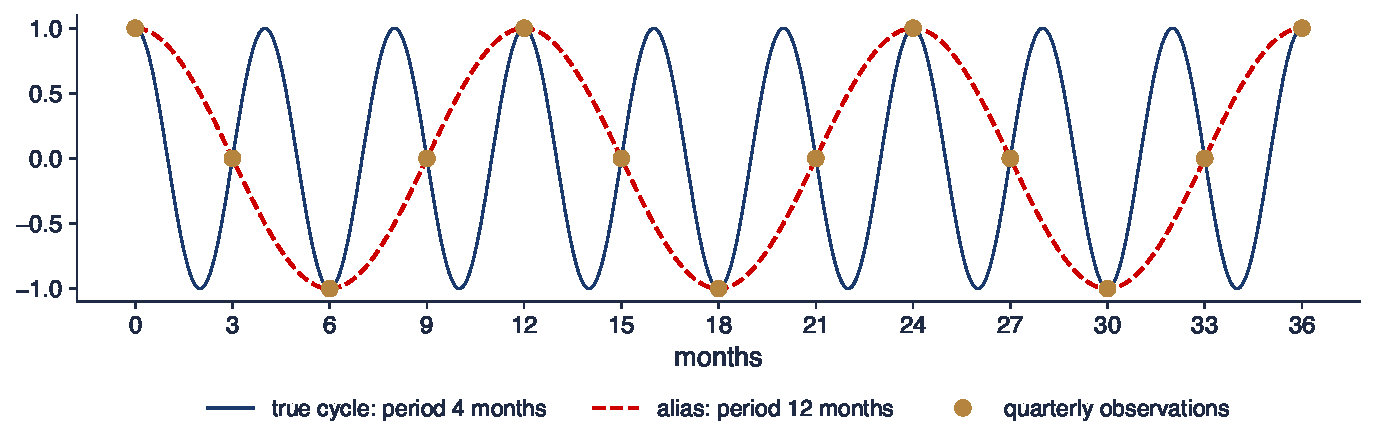
\includegraphics[width=0.97\textwidth,height=0.6\textheight,keepaspectratio]{tsa_ch12_aliasing.pdf}
\end{center}
\vspace{-0.25cm}
\begin{itemize}
    \item A cycle of 4 months ($\nu = 1/4$ per month) observed only once a quarter (every 3 months)
\end{itemize}
\quantlet{TSA\_ch12\_aliasing}{\qlurl{TSA_ch12_aliasing}}
\end{frame}

\begin{frame}{Interpreting aliasing}
\itemsize{\small}
\begin{itemize}
    \item Per quarter, the true frequency is $3 \times 1/4 = 3/4$ cycles, above the Nyquist frequency $1/2$
    \begin{itemize}
        \item it is folded back to $|3/4 - 1| = 1/4$ cycles per quarter: a period of 4 quarters, i.e.\ 12 months
    \end{itemize}
    \item The quarterly points lie exactly on a 12-month wave: the data cannot tell the two cycles apart
    \begin{itemize}
        \item this is \textbf{aliasing}: cycles faster than two observations appear as slower, false cycles
    \end{itemize}
    \item Practical rule: sample at least twice per cycle of interest; average (rather than pick) values when you aggregate to a lower frequency
\end{itemize}
\end{frame}

\begin{frame}{Recap: Cycles and frequencies}
\itemsize{\small}
\begin{itemize}
    \item A cycle has an amplitude, a frequency $\nu$ (cycles per observation), a period $1/\nu$ and a phase
    \item The DFT at the Fourier frequencies $j/T$ rewrites the data as a sum of cycles; Parseval splits the variance by frequency
    \item Only frequencies up to $1/2$ are visible; faster cycles are aliased
\end{itemize}
\end{frame}


%=============================================================================
\section{The spectral density}
%=============================================================================

\begin{frame}{From autocovariances to the spectrum}
\itemsize{\footnotesize}
\begin{itemize}
    \item For a stationary series with autocovariances $\gamma(h)$, $\sum_h|\gamma(h)| < \infty$, the \textbf{spectral density} is
    \begin{itemize}
        \item $f(\nu) = \sum_{h=-\infty}^{\infty}\gamma(h)e^{-2\pi i\nu h} = \gamma(0) + 2\sum_{h=1}^{\infty}\gamma(h)\cos(2\pi\nu h)$, $-1/2 \le \nu \le 1/2$
        \item $\gamma(h) = \mathrm{Cov}(x_t, x_{t+h})$: the autocovariance at lag $h$; $\sum_h|\gamma(h)| < \infty$: the autocovariances die out fast enough (short memory)
        \item in words: $f(\nu)$ is a weighted sum of the autocovariances, with weights $\cos(2\pi\nu h)$ that oscillate at frequency $\nu$
    \end{itemize}
    \item The inverse relation: $\gamma(h) = \int_{-1/2}^{1/2} f(\nu)e^{2\pi i\nu h}\,d\nu$
    \begin{itemize}
        \item the pair $\gamma \leftrightarrow f$ is the \textbf{Wiener--Khinchin} theorem: the autocovariances and the spectrum carry the same information
        \item for $h = 0$: $\mathrm{Var}(x_t) = \gamma(0) = \int_{-1/2}^{1/2} f(\nu)\,d\nu$: the area under $f$ is the variance
    \end{itemize}
    \item Properties: $f(\nu) \ge 0$, $f(-\nu) = f(\nu)$; it is enough to draw $f$ on $[0, 1/2]$
    \begin{itemize}
        \item $f(\nu)\,d\nu$ is the share of the variance due to cycles with frequencies in $[\nu, \nu + d\nu]$
    \end{itemize}
\end{itemize}
\end{frame}

\begin{frame}{White noise, AR(1) and MA(1)}
\itemsize{\footnotesize}
\begin{itemize}
    \item \textbf{White noise} $w_t$, variance $\sigma^2$
    \begin{itemize}
        \item $\gamma(h) = 0$ for $h \ne 0$, so $f(\nu) = \sigma^2$ for every $\nu$
        \item a flat spectrum: all frequencies contribute equally, like white light
    \end{itemize}
    \item \textbf{AR(1)} $x_t = \phi x_{t-1} + w_t$, $|\phi| < 1$
    \begin{itemize}
        \item $f(\nu) = \dfrac{\sigma^2}{1 - 2\phi\cos(2\pi\nu) + \phi^2}$
        \item $\phi$: the autoregressive coefficient; $w_t$: white noise with variance $\sigma^2$
        \item $\phi > 0$: power at low frequencies (smooth, persistent series); $\phi < 0$: power at high frequencies (a zig-zag series)
    \end{itemize}
    \item \textbf{MA(1)} $x_t = w_t + \theta w_{t-1}$
    \begin{itemize}
        \item $f(\nu) = \sigma^2\,[1 + 2\theta\cos(2\pi\nu) + \theta^2]$
        \item $\theta$: the moving-average coefficient; $\theta > 0$ puts power at low frequencies, $\theta < 0$ at high frequencies
        \item directly from the definition: $\gamma(0) = \sigma^2(1 + \theta^2)$, $\gamma(1) = \sigma^2\theta$, so $f = \gamma(0) + 2\gamma(1)\cos(2\pi\nu)$
    \end{itemize}
\end{itemize}
\end{frame}

\begin{frame}{The spectrum of an ARMA model}
\itemsize{\small}
\begin{itemize}
    \item \textbf{ARMA}$(p,q)$
    \begin{itemize}
        \item $\phi(L)x_t = \theta(L)w_t$
        \item $L$: the lag operator, $Lx_t = x_{t-1}$
        \item $\phi(z) = 1 - \phi_1 z - \cdots - \phi_p z^p$ and $\theta(z) = 1 + \theta_1 z + \cdots + \theta_q z^q$: the AR and MA polynomials
    \end{itemize}
    \item Spectral density: the two polynomials evaluated at $z = e^{-2\pi i\nu}$
    \begin{itemize}
        \item $f(\nu) = \sigma^2\dfrac{|\theta(e^{-2\pi i\nu})|^2}{|\phi(e^{-2\pi i\nu})|^2}$
        \item the MA part (numerator) adds power where $|\theta|$ is large; the AR part (denominator) adds power where $|\phi|$ is small
    \end{itemize}
    \item A ratio of two polynomials in $\cos(2\pi\nu)$: smooth and easy to compute (\refBDtm, Sec.~4.4)
\end{itemize}
\end{frame}

\begin{frame}{Worked example: AR(1) and MA(1) spectra}
\itemsize{\small}
\begin{itemize}
    \item AR(1) with $\phi = 0.6$, $\sigma^2 = 1$
    \begin{itemize}
        \item $\nu = 0$: $\cos 0 = 1$, $f(0) = 1/(1 - 0.6)^2 = 1/0.16 = 6.25$
        \item $\nu = 1/2$: $\cos\pi = -1$, $f(1/2) = 1/(1 + 0.6)^2 = 1/2.56 = 0.39$
        \item ratio 16: slow cycles carry far more variance than fast ones
    \end{itemize}
    \item MA(1) with $\theta = 0.5$, $\sigma^2 = 1$
    \begin{itemize}
        \item $f(0) = (1 + 0.5)^2 = 2.25$ and $f(1/2) = (1 - 0.5)^2 = 0.25$
    \end{itemize}
    \item Check of the area for the AR(1): $\int_{-1/2}^{1/2} f = \gamma(0) = 1/(1 - \phi^2) = 1/0.64 = 1.5625$
    \begin{itemize}
        \item the numerical integral of the formula gives the same value
    \end{itemize}
\end{itemize}
\end{frame}

\begin{frame}{AR(2) and pseudo-cycles}
\itemsize{\small}
\begin{itemize}
    \item \textbf{AR(2)} $x_t = \phi_1 x_{t-1} + \phi_2 x_{t-2} + w_t$
    \begin{itemize}
        \item $f(\nu) = \dfrac{\sigma^2}{|1 - \phi_1 e^{-2\pi i\nu} - \phi_2 e^{-4\pi i\nu}|^2}$
        \item with complex roots ($\phi_1^2 + 4\phi_2 < 0$) the ACF is a damped wave and the spectrum has a peak inside $(0, 1/2)$
        \item the peak is at the frequency $\nu^*$ given by $\cos(2\pi\nu^*) = \phi_1(\phi_2 - 1)/(4\phi_2)$, when the right-hand side lies in $[-1, 1]$
    \end{itemize}
    \item A \textbf{pseudo-cycle}
    \begin{itemize}
        \item an irregular cycle whose length and amplitude vary from one round to the next
        \item \refYule\ fitted an AR(2) to Wolfer's sunspot numbers: the first autoregressive model, an alternative to fixed sine waves
    \end{itemize}
    \item Business cycles are pseudo-cycles of this kind: recurrent, but never with the same length (Section 5)
\end{itemize}
\end{frame}

\begin{frame}{Worked example: the peak of an AR(2) spectrum}
\itemsize{\small}
\begin{itemize}
    \item $\phi_1 = 1.5$, $\phi_2 = -0.75$, $\sigma^2 = 1$; complex roots, since $1.5^2 + 4(-0.75) = -0.75 < 0$
    \begin{itemize}
        \item $\cos(2\pi\nu^*) = 1.5 \cdot (-1.75)/(-3) = 0.875$, so $\nu^* = \arccos(0.875)/(2\pi) = 0.0804$
        \item period $1/\nu^* = 12.4$ observations; for yearly data, a cycle of about 12 years
    \end{itemize}
    \item Height: $f(\nu^*) = 64$ against $f(0) = 1/(1 - 1.5 + 0.75)^2 = 16$
    \begin{itemize}
        \item a clear peak: the series oscillates with a typical period of about 12 observations
    \end{itemize}
    \item The same AR(2) is used in Section 4 to test the estimators of the spectrum
\end{itemize}
\end{frame}

\begin{frame}{A gallery of spectral densities}
\itemsize{\footnotesize}
\begin{center}
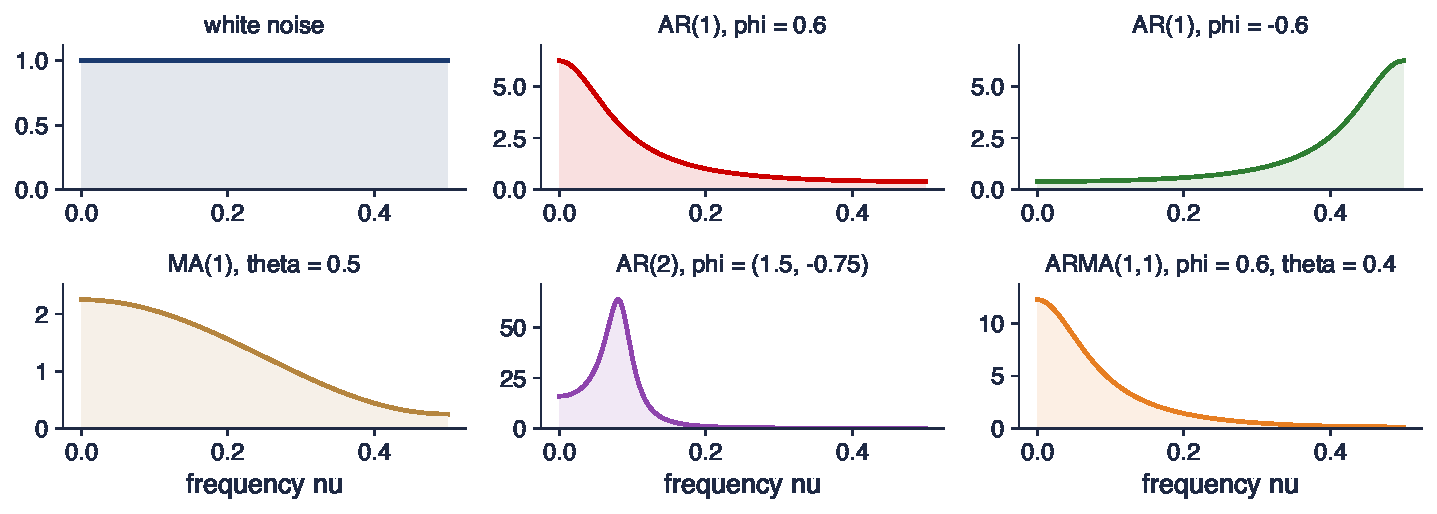
\includegraphics[width=0.97\textwidth,height=0.66\textheight,keepaspectratio]{tsa_ch12_spectra.pdf}
\end{center}
\vspace{-0.25cm}
\begin{itemize}
    \item Theoretical spectra with $\sigma^2 = 1$ on $0 \le \nu \le 1/2$; the shaded area equals half the variance
\end{itemize}
\quantlet{TSA\_ch12\_spectra}{\qlurl{TSA_ch12_spectra}}
\end{frame}

\begin{frame}{Interpreting the gallery}
\itemsize{\small}
\begin{itemize}
    \item Where the power sits tells the type of dependence
    \begin{itemize}
        \item flat: no dependence (white noise); decreasing: positive persistence (AR(1) with $\phi > 0$, MA(1) with $\theta > 0$, ARMA(1,1))
        \item increasing: alternation of signs (AR(1) with $\phi < 0$); a hump inside the band: a pseudo-cycle (AR(2))
    \end{itemize}
    \item The AR(2) concentrates its variance 8.62 in a narrow band around $\nu = 0.0804$
    \begin{itemize}
        \item the ARMA(1,1) adds the MA term to the AR(1): $f(0) = 12.25$, a steeper fall
    \end{itemize}
    \item Reading direction: estimate the spectrum from data, look at its shape, then choose a model whose spectrum looks the same
\end{itemize}
\end{frame}

\begin{frame}{Recap: The spectral density}
\itemsize{\small}
\begin{itemize}
    \item $f(\nu) = \sum_h\gamma(h)e^{-2\pi i\nu h}$; the area under $f$ is the variance; $f$ and the ACF are equivalent
    \item White noise is flat; AR(1) with $\phi > 0$ puts power at low frequencies; AR(2) with complex roots gives a peak
    \item ARMA spectra: $\sigma^2|\theta(e^{-2\pi i\nu})|^2/|\phi(e^{-2\pi i\nu})|^2$
\end{itemize}
\end{frame}


%=============================================================================
\section{The periodogram}
%=============================================================================

\begin{frame}{Arthur Schuster and hidden periodicities}
\itemsize{\small}
\begin{columns}[T]
\begin{column}{0.36\textwidth}
\centering
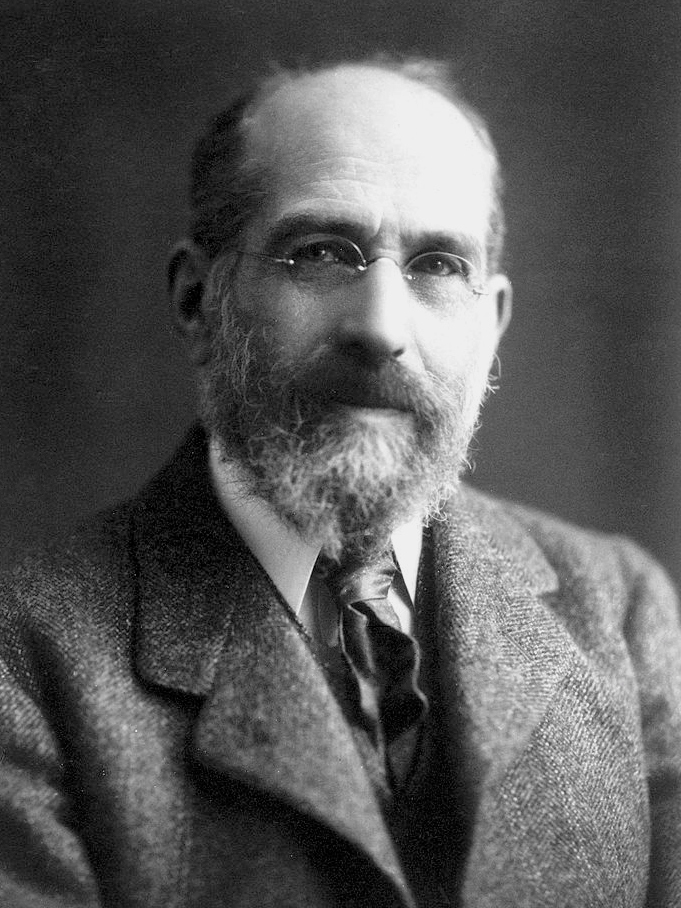
\includegraphics[height=0.5\textheight]{ch12_arthur_schuster.jpg}\\[1mm]
\imgcap{A. Schuster (1851--1934)}
\imgcredit{https://commons.wikimedia.org/wiki/File:Arthur_Schuster.jpg}{Photo: unknown author (1900s); public domain; Wikimedia Commons}
\end{column}
\begin{column}{0.62\textwidth}
\begin{itemize}
    \item \refSchuster\ introduced the \textbf{periodogram} to search for ``hidden periodicities'' in meteorological data
    \begin{itemize}
        \item a claimed 26-day cycle; he showed how to judge whether a peak could be due to chance
    \end{itemize}
    \item Sunspots: counted daily since the 18th century; Rudolf Wolf built the standard index in 1848
    \begin{itemize}
        \item their 11-year cycle is the classic test case of spectral analysis (\tsachlink{https://danpele.github.io/Time-Series-Analysis/EN/Courses/chapter0_introduction.pdf}{Chapter 0})
    \end{itemize}
    \item The question of the section: how do we estimate $f(\nu)$ from one sample, and how reliable is the estimate?
\end{itemize}
\end{column}
\end{columns}
\end{frame}

\begin{frame}{The periodogram}
\itemsize{\small}
\begin{itemize}
    \item \textbf{Periodogram}
    \begin{itemize}
        \item $I(\nu_j) = |d(\nu_j)|^2$ at the Fourier frequencies $\nu_j = j/T$ (after removing the mean)
        \item equivalently $I(\nu_j) = \sum_{|h| < T}\hat\gamma(h)e^{-2\pi i\nu_j h}$: the spectral formula with the sample autocovariances $\hat\gamma(h)$
    \end{itemize}
    \item Regression view: regress $x_t$ on $\cos(2\pi\nu_j t)$ and $\sin(2\pi\nu_j t)$ by OLS, with coefficients $a_j, b_j$
    \begin{itemize}
        \item $I(\nu_j) = \frac{T}{4}(a_j^2 + b_j^2)$: the squared amplitude of the best-fitting cycle at $\nu_j$, scaled by $T/4$
    \end{itemize}
    \item Variance decomposition: $\hat\gamma(0) = \frac{1}{T}\sum_{j=1}^{T-1} I(\nu_j)$
    \begin{itemize}
        \item the share of a band of frequencies is the sum of its ordinates divided by the total
    \end{itemize}
    \item In Python: \texttt{np.abs(np.fft.fft(x - x.mean()))**2 / T}; keep $j = 1, \ldots, \lfloor T/2\rfloor$
\end{itemize}
\end{frame}

\begin{frame}{Sunspots and their periodogram}
\itemsize{\footnotesize}
\begin{center}
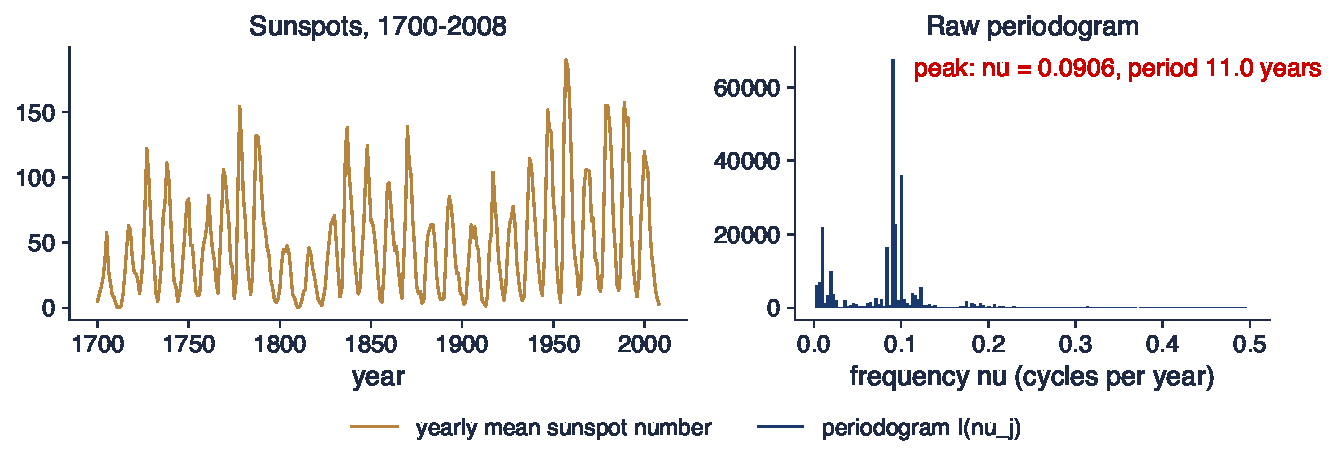
\includegraphics[width=0.97\textwidth,height=0.62\textheight,keepaspectratio]{tsa_ch12_sunspots.pdf}
\end{center}
\vspace{-0.25cm}
\begin{itemize}
    \item Yearly mean sunspot number, 1700--2008, 309 observations (Wolf / SILSO series, statsmodels); right: the raw periodogram
\end{itemize}
\quantlet{TSA\_ch12\_sunspots}{\qlurl{TSA_ch12_sunspots}}
\end{frame}

\begin{frame}{Interpreting the sunspot periodogram}
\itemsize{\small}
\begin{itemize}
    \item The highest ordinate is at $j = 28$: $\nu = 28/309 = 0.0906$ cycles per year, a period of 11.0 years
    \begin{itemize}
        \item the next largest ordinates are at 10.0 and 10.7 years: the cycle is not exactly regular
    \end{itemize}
    \item Periods between 9 and 13 years carry 60\% of the variance
    \begin{itemize}
        \item the small ordinates near $\nu = 0$ reflect slow changes in the height of the cycles (for example the weak cycles around 1800)
    \end{itemize}
    \item The raw periodogram is very spiky: neighbouring ordinates jump up and down; the next slides explain why
\end{itemize}
\end{frame}

\begin{frame}{Statistical properties of the periodogram}
\itemsize{\footnotesize}
\begin{itemize}
    \item For large $T$, at a Fourier frequency $0 < \nu_j < 1/2$ (\refBDtm, Sec.~10.3; \refSS, Sec.~4.3):
    \begin{itemize}
        \item $\dfrac{2I(\nu_j)}{f(\nu_j)} \approx \chi^2_2$: so $E[I(\nu_j)] \approx f(\nu_j)$ (unbiased) and $\mathrm{Var}[I(\nu_j)] \approx f(\nu_j)^2$
        \item $\chi^2_2$: the chi-square distribution with 2 degrees of freedom (mean 2, variance 4); $f(\nu_j)$: the true spectral density
        \item ordinates at different Fourier frequencies are approximately independent
    \end{itemize}
    \item The variance does \textbf{not} shrink when $T$ grows
    \begin{itemize}
        \item the periodogram is \textbf{not a consistent} estimator of $f$
        \item a larger $T$ gives more ordinates (a finer grid), not more precise ones
    \end{itemize}
    \item $\chi^2_2/2$ is an exponential distribution with mean 1: a single ordinate can easily be 3 times the true value
    \begin{itemize}
        \item its 95\% quantile is 3.00: about 1 ordinate in 20 exceeds $3.00\,f(\nu)$ by chance
    \end{itemize}
\end{itemize}
\end{frame}

\begin{frame}{The periodogram of white noise}
\itemsize{\footnotesize}
\begin{center}
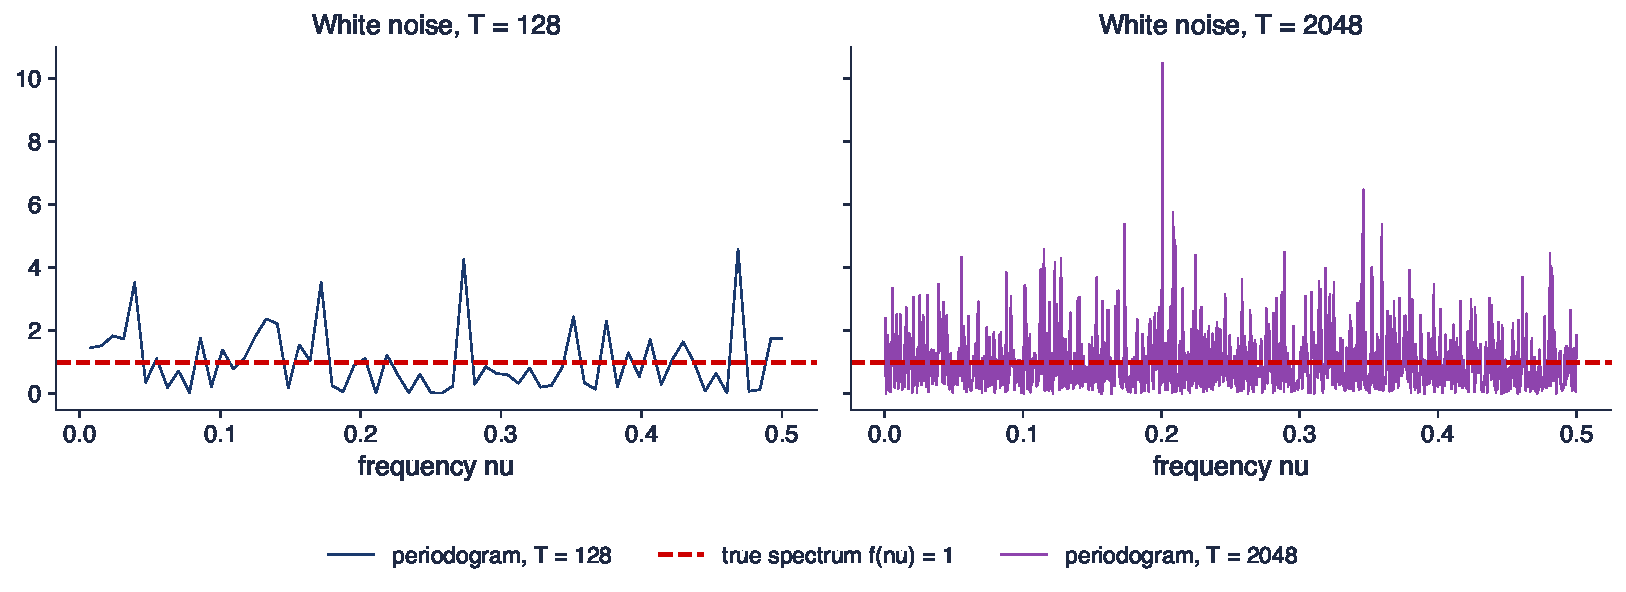
\includegraphics[width=0.97\textwidth,height=0.6\textheight,keepaspectratio]{tsa_ch12_inconsistency.pdf}
\end{center}
\vspace{-0.25cm}
\begin{itemize}
    \item Gaussian white noise with $\sigma^2 = 1$, so the true spectrum is flat at 1; samples of $T = 128$ and $T = 2048$
\end{itemize}
\quantlet{TSA\_ch12\_inconsistency}{\qlurl{TSA_ch12_inconsistency}}
\end{frame}

\begin{frame}{Interpreting the white-noise periodogram}
\itemsize{\small}
\begin{itemize}
    \item $T = 128$: mean of the ordinates 1.03, standard deviation 1.03
    \begin{itemize}
        \item $T = 2048$: mean 1.01, standard deviation 1.00: sixteen times more data, the same scatter
    \end{itemize}
    \item The largest ordinate for $T = 2048$ is 10.5: with 1024 ordinates, isolated tall spikes appear by chance
    \begin{itemize}
        \item a tall spike is not yet a cycle: it needs a test (next slide) or a smoothed estimate (Section 4)
    \end{itemize}
    \item The mean is right (about 1): the periodogram is unbiased but noisy; averaging neighbouring ordinates will reduce the noise
\end{itemize}
\end{frame}

\begin{frame}{Fisher's test of a hidden periodicity (1/2)}
\itemsize{\small}
\begin{itemize}
    \item Hypotheses
    \begin{itemize}
        \item $H_0$: Gaussian white noise; $H_1$: white noise plus one cycle at an unknown Fourier frequency
    \end{itemize}
    \item Statistic of \refFisher: the share of the largest ordinate in the sum of all ordinates
    \begin{itemize}
        \item $g = \max_j I(\nu_j)\,/\,\sum_{j=1}^{m} I(\nu_j)$
        \item $m$: the number of ordinates in $(0, 1/2)$; $\max_j$: the largest of them; $1/m \le g \le 1$
    \end{itemize}
    \item Reading
    \begin{itemize}
        \item under $H_0$ each ordinate is about $1/m$ of the total
        \item a $g$ much larger than $1/m$ signals a cycle: one frequency takes a large share of the variance
    \end{itemize}
\end{itemize}
\end{frame}

\begin{frame}{Fisher's test of a hidden periodicity (2/2)}
\itemsize{\small}
\begin{itemize}
    \item Exact p-value: the probability, under $H_0$, of a $g$ above the observed value $x$
    \begin{itemize}
        \item $P(g > x) = \sum_{k \ge 1,\ kx < 1}(-1)^{k-1}\binom{m}{k}(1 - kx)^{m-1}$
        \item $k$: the summation index, from 1 while $kx < 1$; $\binom{m}{k}$: the binomial coefficient
        \item a small p-value (below 0.05): reject white noise in favour of a cycle
    \end{itemize}
    \item Sunspots: $m = 154$, $g = 0.268$, against $1/m = 0.0065$; p-value $<$\,0.001
    \begin{itemize}
        \item the 11-year peak is far too large to be chance
    \end{itemize}
    \item Caution: $H_0$ is white noise
    \begin{itemize}
        \item against a red (AR(1)-like) background, low-frequency peaks are more likely by chance
        \item so compare with a smooth background spectrum
    \end{itemize}
\end{itemize}
\end{frame}

\begin{frame}{Recap: The periodogram}
\itemsize{\small}
\begin{itemize}
    \item $I(\nu_j) = |d(\nu_j)|^2$: the squared amplitude of the cycle at each Fourier frequency; it sums to the variance
    \item $2I/f \approx \chi^2_2$: unbiased but not consistent; neighbouring ordinates are nearly independent
    \item Sunspots: a peak at 11.0 years; Fisher's $g$ rejects white noise
\end{itemize}
\end{frame}


%=============================================================================
\section{Estimating the spectrum}
%=============================================================================

\begin{frame}{Leakage and tapering}
\itemsize{\footnotesize}
\begin{itemize}
    \item A cycle whose frequency is not a Fourier frequency does not fit a whole number of times in the sample
    \begin{itemize}
        \item cutting the series at $t = 1$ and $t = T$ creates a jump; its power \textbf{leaks} into all other frequencies
        \item leakage from a strong peak can hide a weak cycle elsewhere
    \end{itemize}
    \item \textbf{Tapering}
    \begin{itemize}
        \item multiply the data by a window $h_t$ that goes smoothly to 0 at both ends before the DFT
        \item Hann (cosine bell) window: $h_t = \frac12[1 - \cos(2\pi(t - 0.5)/T)]$, rescaled to keep the total power
        \item $h_t$ is close to 0 at $t = 1$ and $t = T$ and equals 1 in the middle of the sample
        \item the price: a slightly wider main peak (less resolution) for much smaller leakage
    \end{itemize}
    \item Default in practice: always taper a little; always remove the mean (and a trend, if there is one) first
\end{itemize}
\end{frame}

\begin{frame}{Leakage: raw and tapered periodograms}
\itemsize{\footnotesize}
\begin{center}
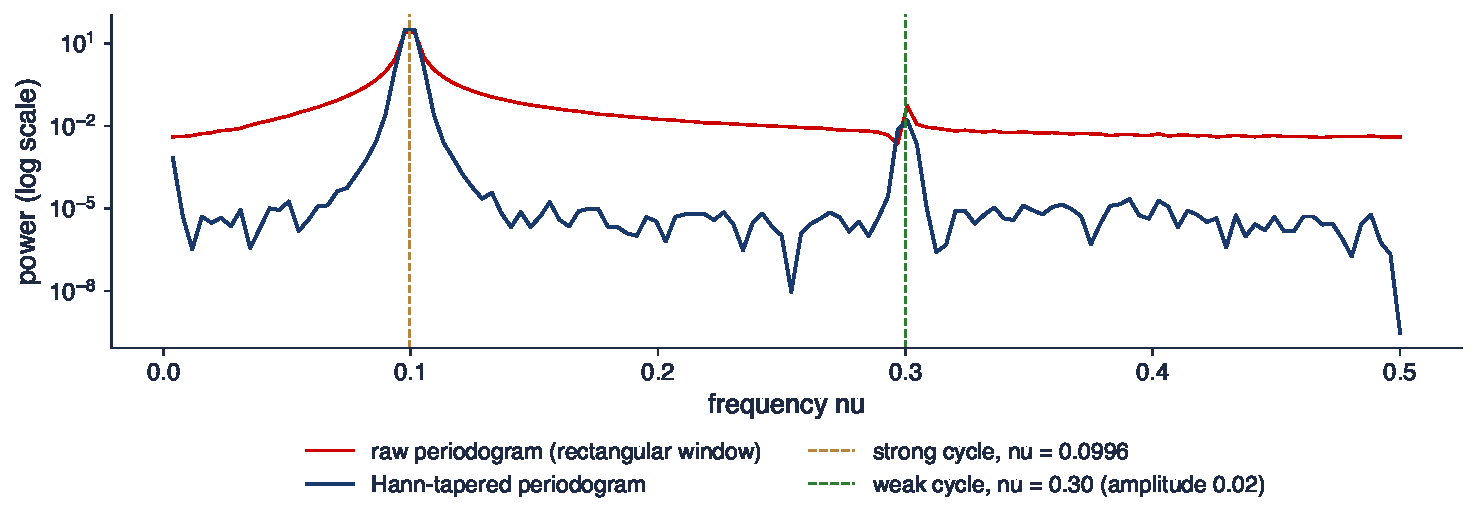
\includegraphics[width=0.97\textwidth,height=0.6\textheight,keepaspectratio]{tsa_ch12_leakage.pdf}
\end{center}
\vspace{-0.25cm}
\begin{itemize}
    \item $T = 256$: $\cos(2\pi\cdot 0.0996\,t)$ (between two Fourier frequencies) plus $0.02\cos(2\pi\cdot 0.3\,t)$ and tiny noise; log scale
\end{itemize}
\quantlet{TSA\_ch12\_leakage}{\qlurl{TSA_ch12_leakage}}
\end{frame}

\begin{frame}{Interpreting leakage}
\itemsize{\small}
\begin{itemize}
    \item Raw periodogram: the strong cycle leaks power everywhere; at $\nu = 0.3$ the weak cycle stands only 7.7 times above the leaked background
    \begin{itemize}
        \item with real noise added, this weak peak would be invisible
    \end{itemize}
    \item Hann taper: the background falls by several orders of magnitude and the weak cycle stands 4\,230 times above it
    \begin{itemize}
        \item the main peak is a little wider: tapering trades resolution for less leakage
    \end{itemize}
    \item Log scale is essential: on a linear scale both curves look like a single spike
\end{itemize}
\end{frame}

\begin{frame}{Smoothing the periodogram (1/2): the Daniell estimator}
\itemsize{\footnotesize}
\begin{itemize}
    \item Idea: $f$ is smooth and the ordinates are nearly independent, so average $L = 2m + 1$ neighbouring ordinates
    \begin{itemize}
        \item \textbf{Daniell} estimator: $\hat f(\nu_j) = \frac{1}{L}\sum_{k=-m}^{m} I(\nu_{j+k})$
        \item $m$: the number of neighbours on each side; $k$: runs from $-m$ to $m$; $\hat f$: the estimated spectrum
        \item variance about $f^2/L$: $L$ times smaller than that of one ordinate
    \end{itemize}
    \item \textbf{Bandwidth} $B = L/T$
    \begin{itemize}
        \item the width of the frequency band that is averaged
    \end{itemize}
    \item Bias--variance trade-off: a larger $L$ lowers the variance but flattens narrow peaks (bias)
    \begin{itemize}
        \item consistency needs $L \to \infty$ and $L/T \to 0$, e.g.\ $L \approx \sqrt T$
    \end{itemize}
\end{itemize}
\end{frame}

\begin{frame}{Smoothing the periodogram (2/2): lag windows and Welch}
\itemsize{\small}
\begin{itemize}
    \item Equivalent view: smoothing in frequency $=$ down-weighting distant autocovariances (lag windows)
    \begin{itemize}
        \item Bartlett window: $\hat f(\nu) = \sum_{|h| \le M}(1 - |h|/M)\hat\gamma(h)e^{-2\pi i\nu h}$ (\refBartlett; \refBT)
        \item $M$: the truncation lag; autocovariances beyond lag $M$ are dropped, the others get weights $1 - |h|/M$ that fall linearly
        \item a smaller $M$ means more smoothing
    \end{itemize}
    \item The \textbf{Welch} method (\refWelch)
    \begin{itemize}
        \item an average of the periodograms of $K$ segments
        \item split the series into $K$ overlapping segments, taper each, average their periodograms
        \item \texttt{scipy.signal.welch}; the segment length sets the resolution
    \end{itemize}
\end{itemize}
\end{frame}

\begin{frame}{Smoothed estimates of an AR(2) spectrum}
\itemsize{\footnotesize}
\begin{center}
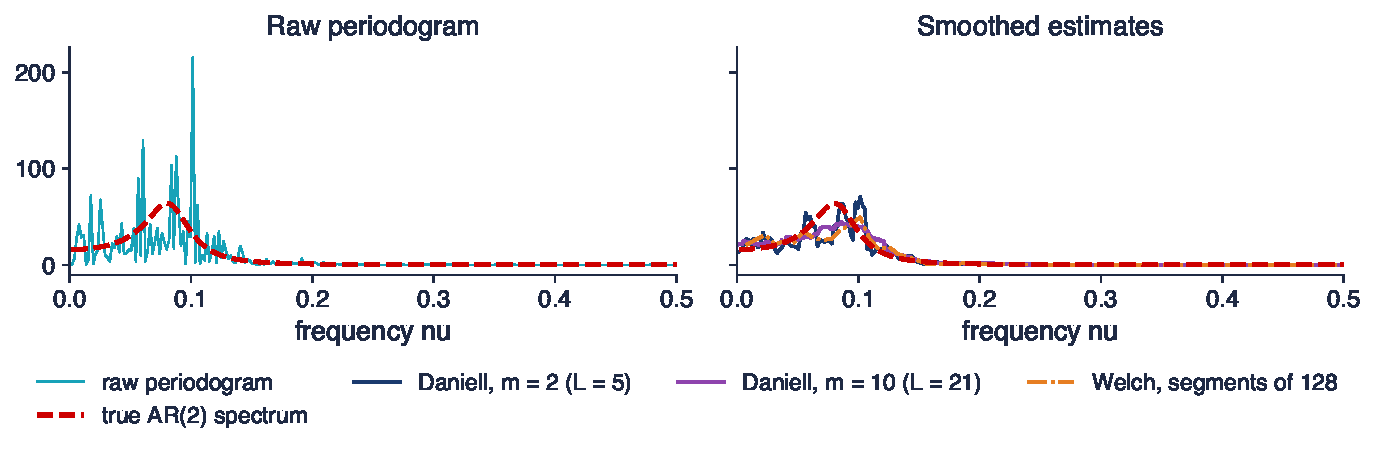
\includegraphics[width=0.97\textwidth,height=0.6\textheight,keepaspectratio]{tsa_ch12_smoothing.pdf}
\end{center}
\vspace{-0.25cm}
\begin{itemize}
    \item Simulated AR(2), $\phi = (1.5, -0.75)$, $T = 512$; true spectrum (dashed) with the raw periodogram (left) and three smoothed estimates (right)
\end{itemize}
\quantlet{TSA\_ch12\_smoothing}{\qlurl{TSA_ch12_smoothing}}
\end{frame}

\begin{frame}{Interpreting the smoothed estimates}
\itemsize{\small}
\begin{itemize}
    \item True peak at $\nu = 0.080$; the highest raw ordinate is at $\nu = 0.102$: a single noisy ordinate misplaces the peak
    \begin{itemize}
        \item peak of Daniell $m = 2$: $\nu = 0.102$; of Daniell $m = 10$: $\nu = 0.086$; of Welch ($K = 7$ segments of 128): $\nu = 0.102$
    \end{itemize}
    \item Mean squared error of $\log\hat f$: raw 1.86; Daniell $m = 2$: 0.25; $m = 10$: 0.09; Welch: 0.24
    \begin{itemize}
        \item the price of heavy smoothing: the peak height drops from 64 to 44 (bias)
    \end{itemize}
    \item Choose the bandwidth by looking at several values: keep the narrowest one whose estimate is no longer dominated by noise
\end{itemize}
\end{frame}

\begin{frame}{Confidence bands for the spectrum}
\itemsize{\footnotesize}
\begin{itemize}
    \item Daniell estimate with $L$ terms: $\dfrac{2L\,\hat f(\nu)}{f(\nu)} \approx \chi^2_{2L}$ (degrees of freedom $df = 2L$)
    \begin{itemize}
        \item 95\% interval: $\left[\dfrac{df\,\hat f(\nu)}{\chi^2_{df}(0.975)},\ \dfrac{df\,\hat f(\nu)}{\chi^2_{df}(0.025)}\right]$
        \item $\chi^2_{df}(p)$: the quantile of level $p$ of the chi-square distribution with $df$ degrees of freedom
    \end{itemize}
    \item The interval is a fixed multiple of $\hat f$: on a log scale its width is the same at every frequency
    \begin{itemize}
        \item a peak is significant if the band at the peak lies above the band of the background around it
    \end{itemize}
    \item Welch with $K$ non-overlapping segments: $df \approx 2K$; overlap and tapering change $df$ a little
\end{itemize}
\end{frame}

\begin{frame}{Worked example: a 95\% band with $L = 5$}
\itemsize{\small}
\begin{itemize}
    \item $L = 5$ ($m = 2$), so $df = 10$; from the $\chi^2_{10}$ table: $\chi^2_{10}(0.025) = 3.25$ and $\chi^2_{10}(0.975) = 20.48$
    \begin{itemize}
        \item lower bound: $10/20.48 = 0.49$ times $\hat f$; upper bound: $10/3.25 = 3.08$ times $\hat f$
    \end{itemize}
    \item Sunspots: at the smoothed peak (period 10.3 years) $\hat f = 26\,095$
    \begin{itemize}
        \item 95\% interval: [12\,740, 80\,367]: asymmetric, wider upwards
    \end{itemize}
    \item With only 5 ordinates the estimate is still uncertain by a factor of 2--3; more smoothing narrows the band but blurs the peak
\end{itemize}
\end{frame}

\begin{frame}{Sunspots: smoothed spectrum with a confidence band}
\itemsize{\footnotesize}
\begin{center}
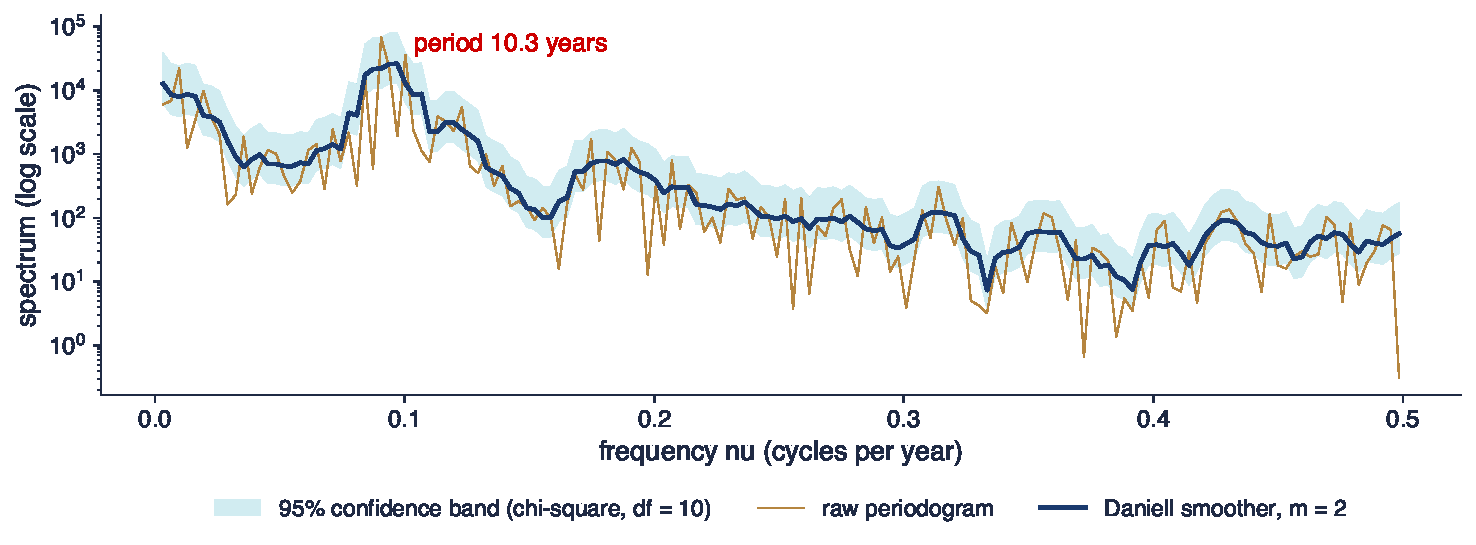
\includegraphics[width=0.97\textwidth,height=0.6\textheight,keepaspectratio]{tsa_ch12_sunspot_ci.pdf}
\end{center}
\vspace{-0.25cm}
\begin{itemize}
    \item Daniell smoother with $m = 2$ ($L = 5$, $df = 10$, bandwidth $B = 5/309 = 0.016$ cycles per year) and its 95\% band; log scale
\end{itemize}
\quantlet{TSA\_ch12\_sunspot\_ci}{\qlurl{TSA_ch12_sunspot_ci}}
\end{frame}

\begin{frame}{Interpreting the smoothed sunspot spectrum}
\itemsize{\small}
\begin{itemize}
    \item The band at the peak (period 10.3 years) lies entirely above the band of the background at higher frequencies
    \begin{itemize}
        \item the 11-year cycle is a robust feature, not a chance spike
    \end{itemize}
    \item A second, smaller hump near $\nu \approx 0.18$ (about 5.5 years) is the first \textbf{harmonic}
    \begin{itemize}
        \item the sunspot cycle is not a sine wave: it rises fast and decays slowly, and a non-sinusoidal cycle has power at multiples of its frequency
    \end{itemize}
    \item Power also rises towards $\nu = 0$: the height of the cycles changes over decades and centuries
\end{itemize}
\end{frame}

\begin{frame}{Recap: Estimating the spectrum}
\itemsize{\small}
\begin{itemize}
    \item Taper to reduce leakage; plot spectra on a log scale
    \item Smooth over $L$ ordinates (Daniell, Bartlett, Welch): variance $\approx f^2/L$, but narrow peaks are flattened
    \item 95\% band: $[df\,\hat f/\chi^2_{df}(0.975),\ df\,\hat f/\chi^2_{df}(0.025)]$ with $df = 2L$
\end{itemize}
\end{frame}


%=============================================================================
\section{Cycles in economic and energy data}
%=============================================================================

\begin{frame}{The typical spectral shape and the business cycle}
\itemsize{\small}
\begin{itemize}
    \item \refGranger: the spectrum of most economic levels (GDP, prices) falls steeply from $\nu = 0$: the \textbf{typical spectral shape}
    \begin{itemize}
        \item trends and near unit roots put almost all the variance at the lowest frequencies and hide the cycles
        \item so we first make the series stationary: growth rates (differences) or a detrended cycle
    \end{itemize}
    \item \textbf{Business-cycle band}
    \begin{itemize}
        \item fluctuations lasting 1.5 to 8 years, i.e.\ 6 to 32 quarters (\refBK)
        \item in frequency: $1/32 \le \nu \le 1/6$ cycles per quarter
    \end{itemize}
    \item Data: US real GDP (FRED GDPC1, 291 quarterly growth rates) and Romanian real GDP (Eurostat, seasonally adjusted, 99 growth rates)
    \begin{itemize}
        \item both up to 2019 Q4: the 2020 collapse and rebound would dominate every periodogram
        \item the cycle is also extracted with the HP filter, $\lambda = 1600$ (\refHPf; \tsachlink{https://danpele.github.io/Time-Series-Analysis/EN/Courses/chapter10_state_space_kalman_markov_switching.pdf}{Chapter 10})
    \end{itemize}
\end{itemize}
\end{frame}

\begin{frame}{GDP growth and HP cycles}
\itemsize{\footnotesize}
\begin{center}
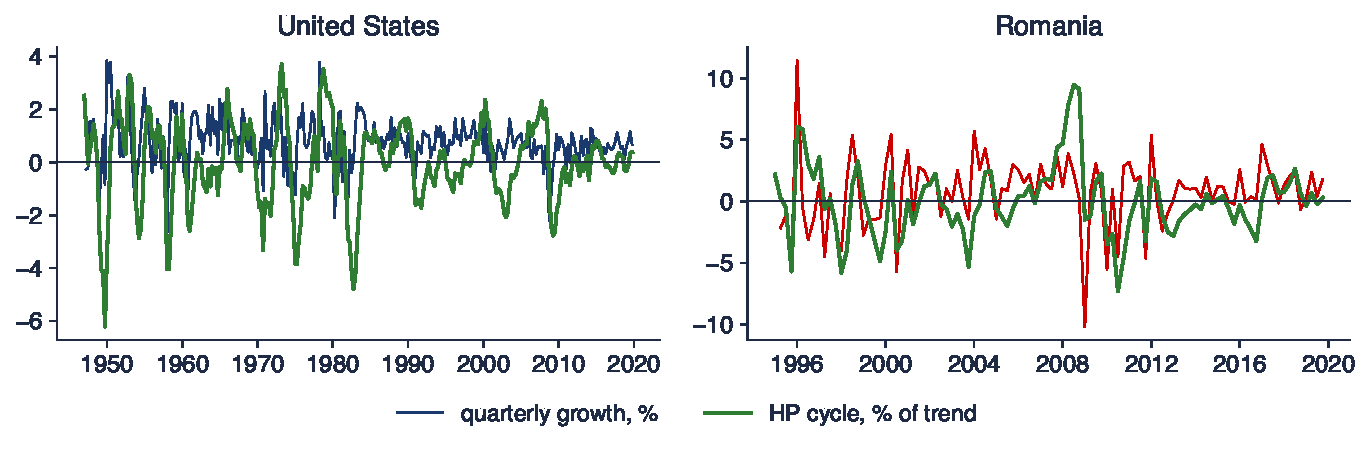
\includegraphics[width=0.97\textwidth,height=0.6\textheight,keepaspectratio]{tsa_ch12_gdp_series.pdf}
\end{center}
\vspace{-0.25cm}
\begin{itemize}
    \item Quarterly growth $100\,\Delta\ln \mathrm{GDP}_t$ and the HP cycle ($100\ln\mathrm{GDP}_t$ minus its HP trend), United States 1947--2019 and Romania 1995--2019
\end{itemize}
\quantlet{TSA\_ch12\_gdp\_series}{\qlurl{TSA_ch12_gdp_series}}
\end{frame}

\begin{frame}{Interpreting the GDP series}
\itemsize{\small}
\begin{itemize}
    \item United States: mean growth 0.78\% per quarter, standard deviation 0.93; HP cycle standard deviation 1.58\% of trend
    \begin{itemize}
        \item the cycle shows the recessions as deep troughs (1958, 1975, 1982, 2009)
    \end{itemize}
    \item Romania: mean growth 0.73\%, standard deviation 2.85: three times more volatile
    \begin{itemize}
        \item one large boom--bust (2004--2010) dominates a sample of only 25 years
    \end{itemize}
    \item The growth rate is noisy and short-lived; the HP cycle is smooth and persistent: their spectra will differ
\end{itemize}
\end{frame}

\begin{frame}{Spectra of GDP growth and HP cycles}
\itemsize{\footnotesize}
\begin{center}
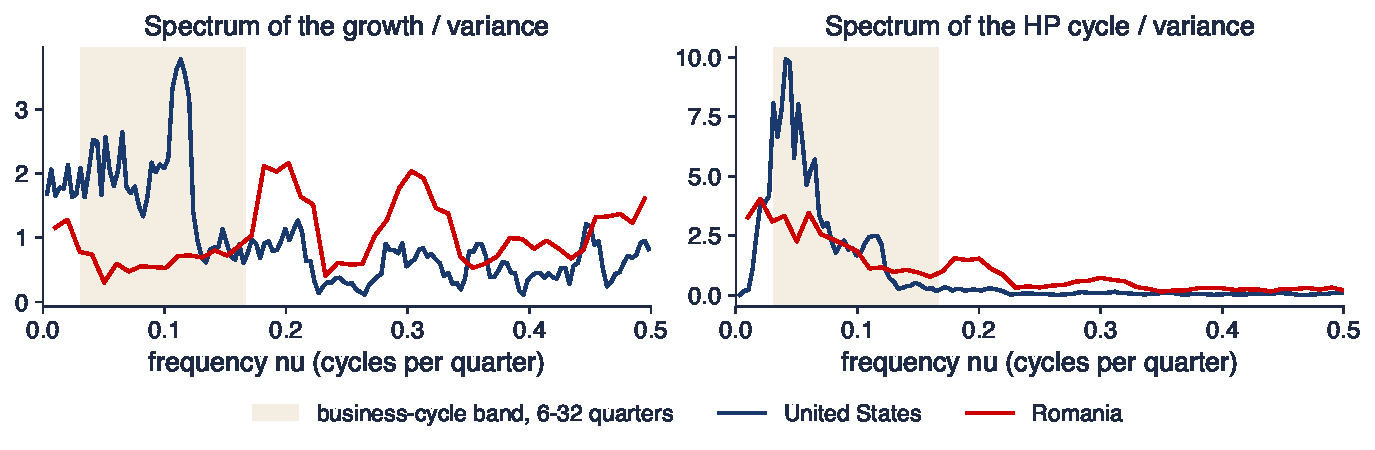
\includegraphics[width=0.97\textwidth,height=0.6\textheight,keepaspectratio]{tsa_ch12_gdp_spectra.pdf}
\end{center}
\vspace{-0.25cm}
\begin{itemize}
    \item Daniell smoother, $m = 2$; each spectrum divided by the variance of its series; shaded: periods of 6 to 32 quarters
\end{itemize}
\quantlet{TSA\_ch12\_gdp\_spectra}{\qlurl{TSA_ch12_gdp_spectra}}
\end{frame}

\begin{frame}{Interpreting the GDP spectra}
\itemsize{\small}
\begin{itemize}
    \item US growth: 49\% of the variance in the business-cycle band; the smoothed peak is at about 8.8 quarters
    \begin{itemize}
        \item Romanian growth: only 16\%; most of its variance is at high frequencies (quarter-to-quarter noise and revisions)
    \end{itemize}
    \item US HP cycle: 80\% of the variance in the band, peak at 24.3 quarters (about 6.1 years)
    \begin{itemize}
        \item Romanian HP cycle: 49\% in the band and 17\% at periods longer than 8 years: one long cycle in a short sample
    \end{itemize}
    \item Caution: the HP filter itself removes low frequencies and can shape the peak (Section 7); 99 Romanian observations give a very wide confidence band
\end{itemize}
\end{frame}

\begin{frame}{The rhythm of electricity demand}
\itemsize{\footnotesize}
\begin{center}
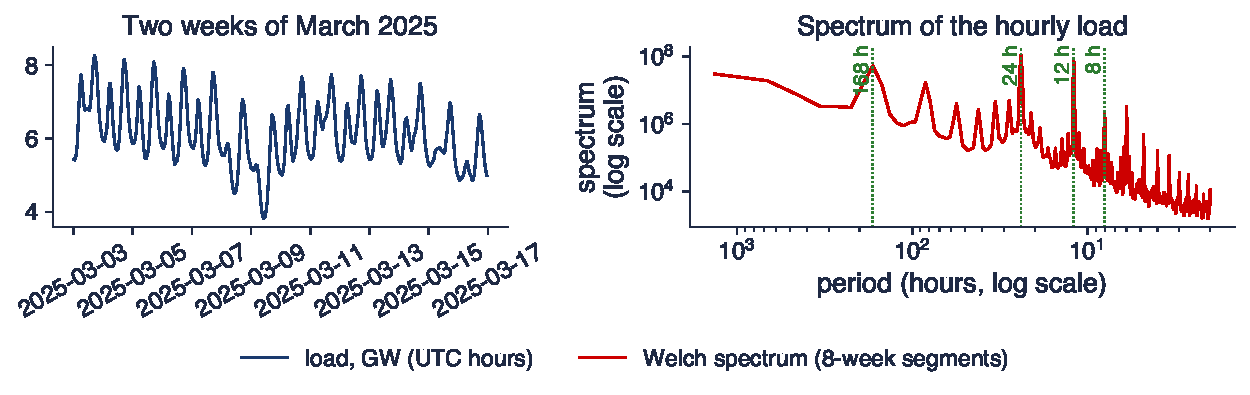
\includegraphics[width=0.97\textwidth,height=0.58\textheight,keepaspectratio]{tsa_ch12_load.pdf}
\end{center}
\vspace{-0.25cm}
\begin{itemize}
    \item Hourly electricity load of Romania (ENTSO-E, MW, UTC hours), 2022--2026, 39\,408 hours, mean 6\,176 MW (\tsachlink{https://danpele.github.io/Time-Series-Analysis/EN/Courses/chapter4_seasonality_forecasting.pdf}{Chapter 4}); Welch spectrum with 8-week segments
\end{itemize}
\quantlet{TSA\_ch12\_load}{\qlurl{TSA_ch12_load}}
\end{frame}

\begin{frame}{Interpreting the load spectrum}
\itemsize{\small}
\begin{itemize}
    \item Sharp peaks at 24, 12 and 8 hours: the daily cycle and its harmonics (morning and evening peaks are not a sine wave)
    \begin{itemize}
        \item the daily cycle and its harmonics hold 34\% of the variance
    \end{itemize}
    \item A peak at 167.7 hours (one week) and its harmonic at 84.0 hours: working days against weekends
    \begin{itemize}
        \item weekly components: 16\%; periods longer than a month (winter against summer): 33\%
    \end{itemize}
    \item This is why \tsachlink{https://danpele.github.io/Time-Series-Analysis/EN/Courses/chapter4_seasonality_forecasting.pdf}{Chapter 4} modelled the load with daily and weekly Fourier terms: the spectrum shows which periods to include
\end{itemize}
\end{frame}

\begin{frame}{Recap: Cycles in data}
\itemsize{\small}
\begin{itemize}
    \item Remove trends first (growth rates, detrended cycles): levels have the typical spectral shape
    \item US GDP: a business-cycle peak of about 6.1 years in the HP cycle; Romania: too short a sample for a sharp answer
    \item Electricity load: daily and weekly cycles with harmonics; the spectrum chooses the Fourier terms of a forecasting model
\end{itemize}
\end{frame}


%=============================================================================
\section{Long memory: the pole at zero}
%=============================================================================

\begin{frame}{Long memory in the frequency domain (1/2)}
\itemsize{\footnotesize}
\begin{itemize}
    \item \tsachlink{https://danpele.github.io/Time-Series-Analysis/EN/Courses/chapter8_long_memory_arfima.pdf}{Chapter 8}: a long-memory series has autocorrelations that decay like a power of the lag
    \begin{itemize}
        \item $\rho(h) \sim Ch^{2d-1}$: $\rho(h)$ is the autocorrelation at lag $h$, $C > 0$ a constant, $\sim$ means ``proportional for large $h$''
        \item $d$: the memory parameter; $0 < d < 1/2$ gives stationary long memory; then $\sum_h\gamma(h) = \infty$ and $f(0) = \infty$
    \end{itemize}
    \item ARFIMA$(0,d,0)$: the spectrum explodes at zero
    \begin{itemize}
        \item $f(\nu) = \sigma^2\,|2\sin(\pi\nu)|^{-2d} \approx \sigma^2(2\pi\nu)^{-2d}$ near $\nu = 0$: a \textbf{pole} at zero
        \item taking logs: $\log f(\nu) \approx \log\sigma^2 - 2d\log(2\pi\nu)$, a straight line in $\log\nu$ with slope $-2d$
    \end{itemize}
    \item Short memory (ARMA) has a finite $f(0)$: the log--log plot flattens at low frequencies
\end{itemize}
\end{frame}

\begin{frame}{Long memory in the frequency domain (2/2): the GPH estimator}
\itemsize{\small}
\begin{itemize}
    \item \refGPH: a regression of the log-periodogram on a log-frequency term
    \begin{itemize}
        \item regress $\log I(\nu_j)$ on $-\log(4\sin^2(\pi\nu_j))$ for $j = 1, \ldots, m$; the slope is $\hat d$
        \item standard error $\pi/\sqrt{24m}$: it shrinks as more frequencies are used
    \end{itemize}
    \item Only the lowest $m = \lfloor T^{0.65}\rfloor$ frequencies are used, where the pole dominates
    \begin{itemize}
        \item a larger $m$ lowers the standard error but brings in short-memory effects (bias)
    \end{itemize}
    \item Reading
    \begin{itemize}
        \item $\hat d$ close to 0: short memory; $0 < \hat d < 0.5$: stationary long memory; $\hat d \ge 0.5$: nonstationary
    \end{itemize}
\end{itemize}
\end{frame}

\begin{frame}{The pole at zero in stock-market data}
\itemsize{\footnotesize}
\begin{center}
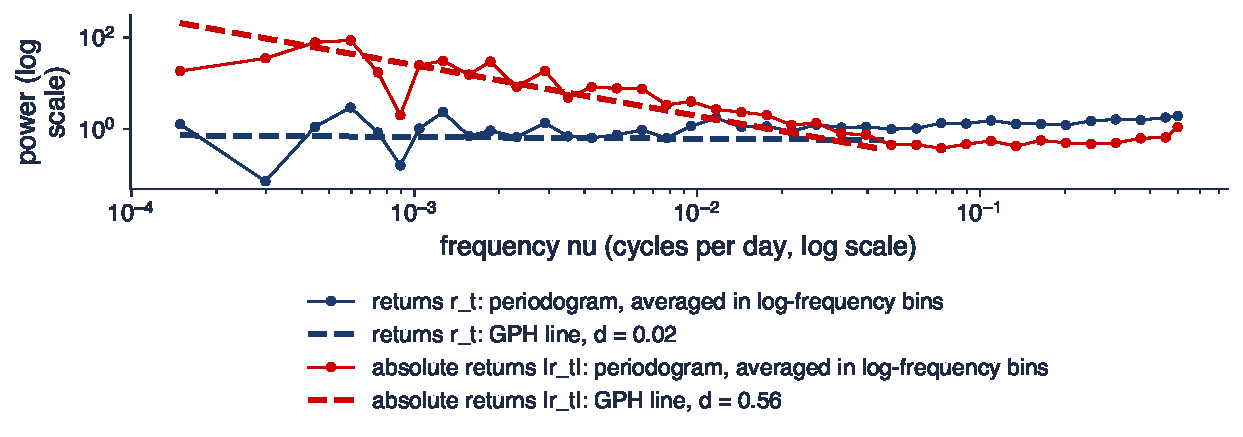
\includegraphics[width=0.97\textwidth,height=0.58\textheight,keepaspectratio]{tsa_ch12_long_memory.pdf}
\end{center}
\vspace{-0.25cm}
\begin{itemize}
    \item Daily S\&P 500 log returns, 2000--2026, $T = 6\,714$ (EODHD); periodogram averaged in 40 log-frequency bins; GPH lines on the lowest $m = 307$ frequencies (periods above 22 days)
\end{itemize}
\quantlet{TSA\_ch12\_long\_memory}{\qlurl{TSA_ch12_long_memory}}
\end{frame}

\begin{frame}{Interpreting the log--log periodogram}
\itemsize{\small}
\begin{itemize}
    \item Returns $r_t$: flat at low frequencies, GPH $\hat d = 0.02$ (standard error 0.037): no long memory in the returns
    \begin{itemize}
        \item a flat spectrum is what market efficiency predicts for returns (\tsachlink{https://danpele.github.io/Time-Series-Analysis/EN/Courses/chapter1_stochastic_processes_stationarity.pdf}{Chapter 1})
    \end{itemize}
    \item Absolute returns $|r_t|$: power rises steadily towards $\nu = 0$, slope $-2\hat d$ with $\hat d = 0.56$
    \begin{itemize}
        \item the long memory of volatility (\tsachlink{https://danpele.github.io/Time-Series-Analysis/EN/Courses/chapter8_long_memory_arfima.pdf}{Chapter 8}); $\hat d$ near or above 0.5 also reflects breaks such as 2008 and 2020
    \end{itemize}
    \item The same spectral picture explains why GPH and local Whittle (\tsachlink{https://danpele.github.io/Time-Series-Analysis/EN/Courses/chapter8_long_memory_arfima.pdf}{Chapter 8}) are frequency-domain estimators
\end{itemize}
\end{frame}


%=============================================================================
\section{Linear filters}
%=============================================================================

\begin{frame}{Linear filters and their gain (1/2)}
\itemsize{\small}
\begin{itemize}
    \item A \textbf{linear filter} turns an input series $x_t$ into an output $y_t$ by a weighted sum of current and past values
    \begin{itemize}
        \item $y_t = \sum_j a_j x_{t-j}$; $a_j$: the filter weights; $j$: the lag
    \end{itemize}
    \item Its \textbf{frequency response} is $A(\nu) = \sum_j a_j e^{-2\pi i\nu j}$
    \begin{itemize}
        \item key result: $f_y(\nu) = |A(\nu)|^2 f_x(\nu)$; $f_x$, $f_y$: the spectra of input and output
        \item $|A(\nu)|^2$ is the \textbf{squared gain}: above 1 the filter amplifies cycles of frequency $\nu$, below 1 it damps them, 0 removes them
    \end{itemize}
\end{itemize}
\end{frame}

\begin{frame}{Linear filters and their gain (2/2)}
\itemsize{\small}
\begin{itemize}
    \item First difference $y_t = x_t - x_{t-1}$: $|A(\nu)|^2 = |1 - e^{-2\pi i\nu}|^2 = 4\sin^2(\pi\nu)$
    \begin{itemize}
        \item zero at $\nu = 0$ (removes the trend), 4 at $\nu = 1/2$ (amplifies noise); at a period of 40 quarters: 0.025; at 4 quarters: 2
    \end{itemize}
    \item Seasonal difference $(1 - L^4)x_t = x_t - x_{t-4}$ (quarterly data): squared gain $4\sin^2(4\pi\nu)$
    \begin{itemize}
        \item zero at $\nu = 0, 1/4, 1/2$: it removes the trend and the seasonal cycles
    \end{itemize}
    \item HP cycle filter: squared gain $\dfrac{4\lambda(1 - \cos 2\pi\nu)^2}{1 + 4\lambda(1 - \cos 2\pi\nu)^2}$
    \begin{itemize}
        \item $\lambda$: the smoothing parameter (1600 for quarterly data); a larger $\lambda$ moves the cut-off to slower cycles
        \item close to 0 at low frequencies, close to 1 at high ones: a \textbf{high-pass} filter
    \end{itemize}
\end{itemize}
\end{frame}

\begin{frame}{Squared gains of common filters}
\itemsize{\footnotesize}
\begin{center}
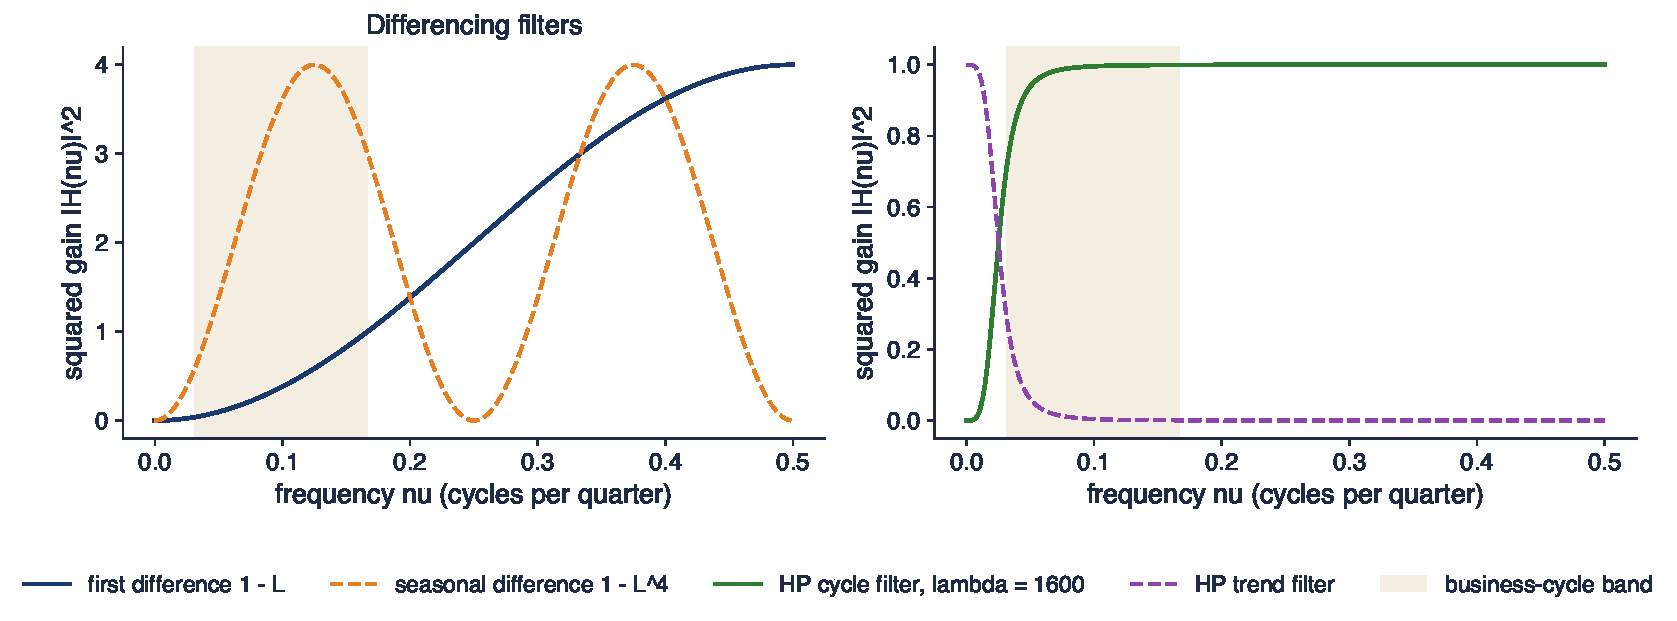
\includegraphics[width=0.97\textwidth,height=0.6\textheight,keepaspectratio]{tsa_ch12_filters.pdf}
\end{center}
\vspace{-0.25cm}
\begin{itemize}
    \item Left: first difference and seasonal difference ($s = 4$); right: HP cycle and trend filters, $\lambda = 1600$ (quarterly data); shaded: 6--32 quarters
\end{itemize}
\quantlet{TSA\_ch12\_filters}{\qlurl{TSA_ch12_filters}}
\end{frame}

\begin{frame}{Interpreting the filter gains}
\itemsize{\small}
\begin{itemize}
    \item Differencing is not neutral: it weakens business cycles and amplifies the highest frequencies
    \begin{itemize}
        \item this is why growth rates look noisier than levels; filtering white noise can even create spurious cycles (the Slutsky effect, \tsachlink{https://danpele.github.io/Time-Series-Analysis/EN/Courses/chapter0_introduction.pdf}{Chapter 0})
    \end{itemize}
    \item HP cycle filter: gain 0.998 at 8 quarters, 0.70 at 32 quarters, 0.49 at 40 quarters; half power at about 40 quarters
    \begin{itemize}
        \item it keeps everything faster than 10 years, including noise: not a band-pass filter (\refBK)
    \end{itemize}
    \item Applied to a random walk, the HP filter produces a cycle with a peak that comes from the filter, not from the data (\refHamHP)
\end{itemize}
\end{frame}


%=============================================================================
\section{Two series: coherence and phase}
%=============================================================================

\begin{frame}{Cross-spectrum, coherence and phase}
\itemsize{\footnotesize}
\begin{itemize}
    \item For two stationary series with cross-covariances $\gamma_{xy}(h) = \mathrm{Cov}(x_{t+h}, y_t)$:
    \begin{itemize}
        \item \textbf{cross-spectrum} $f_{xy}(\nu) = \sum_h\gamma_{xy}(h)e^{-2\pi i\nu h}$, a complex number at each frequency
        \item $f_x$, $f_y$: the spectra of $x$ and $y$ separately
    \end{itemize}
    \item \textbf{Squared coherence}
    \begin{itemize}
        \item $\rho^2_{xy}(\nu) = \dfrac{|f_{xy}(\nu)|^2}{f_x(\nu)f_y(\nu)} \in [0, 1]$
        \item a squared correlation frequency by frequency: how well the cycles of $x$ and $y$ at $\nu$ move together
    \end{itemize}
    \item \textbf{Phase} $\varphi(\nu) = \arg f_{xy}(\nu)$
    \begin{itemize}
        \item the shift between the two cycles, in radians
        \item $\arg$: the angle of a complex number in the plane (its argument)
        \item a time lag of $k$ periods gives a phase that is linear in frequency: $\varphi(\nu) = \pm 2\pi\nu k$; so the lag is $|\varphi|/(2\pi\nu)$
    \end{itemize}
    \item Estimation: smooth the cross-periodogram like the periodogram; the raw coherence is always 1, so smoothing is compulsory
\end{itemize}
\end{frame}

\begin{frame}{Industrial production and unemployment}
\itemsize{\footnotesize}
\begin{center}
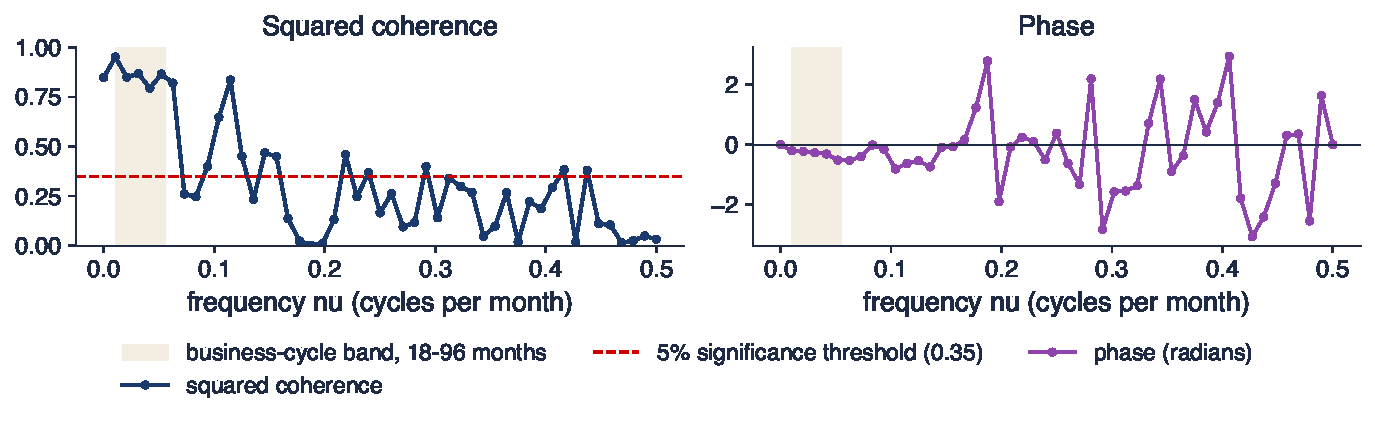
\includegraphics[width=0.97\textwidth,height=0.56\textheight,keepaspectratio]{tsa_ch12_coherence.pdf}
\end{center}
\vspace{-0.25cm}
\begin{itemize}
    \item US monthly data, 1948--2019 (FRED INDPRO, UNRATE), $T = 863$: $x_t = 100\,\Delta\ln \mathrm{IP}_t$ and $y_t = -\Delta u_t$ (the fall in the unemployment rate); Welch with $K = 8$ segments of 96 months
\end{itemize}
\quantlet{TSA\_ch12\_coherence}{\qlurl{TSA_ch12_coherence}}
\end{frame}

\begin{frame}{Interpreting coherence and phase}
\itemsize{\small}
\begin{itemize}
    \item In the business-cycle band (18--96 months) the squared coherence averages 0.87 (maximum 0.95), far above the 5\% threshold 0.35
    \begin{itemize}
        \item at frequencies faster than 6 months it averages only 0.17: the monthly noise of the two series is unrelated
        \item the ordinary correlation, 0.49, mixes the strong link of the cycles with the weak link of the noise
    \end{itemize}
    \item Phase at the 48-month cycle: -0.23 radians, a lag of about 1.7 months
    \begin{itemize}
        \item the fall in unemployment follows the recovery of production with a short delay (Okun's law, with a lag)
    \end{itemize}
    \item Where the coherence is low, the phase is meaningless: read the phase only in bands with significant coherence
\end{itemize}
\end{frame}


%=============================================================================
\section{A pointer: wavelets}
%=============================================================================

\begin{frame}{Wavelets: frequency that changes over time}
\itemsize{\small}
\begin{itemize}
    \item The spectrum assumes stationarity: the same cycles at every date
    \begin{itemize}
        \item the \textbf{short-time Fourier transform} (STFT) computes spectra in moving windows of fixed length
    \end{itemize}
    \item A \textbf{wavelet} is a short wave packet; the \textbf{continuous wavelet transform} (CWT) stretches it to each period and slides it along the series
    \begin{itemize}
        \item the result, the \textbf{scalogram}, shows the power at each period and each date (\refTC)
        \item short windows for fast cycles, long windows for slow cycles: good resolution at all scales
    \end{itemize}
    \item Beyond this course; a natural project topic (Python: \texttt{pywt}, or the Morlet code of this chapter)
\end{itemize}
\end{frame}

\begin{frame}{Wavelet power of the sunspots}
\itemsize{\footnotesize}
\begin{center}
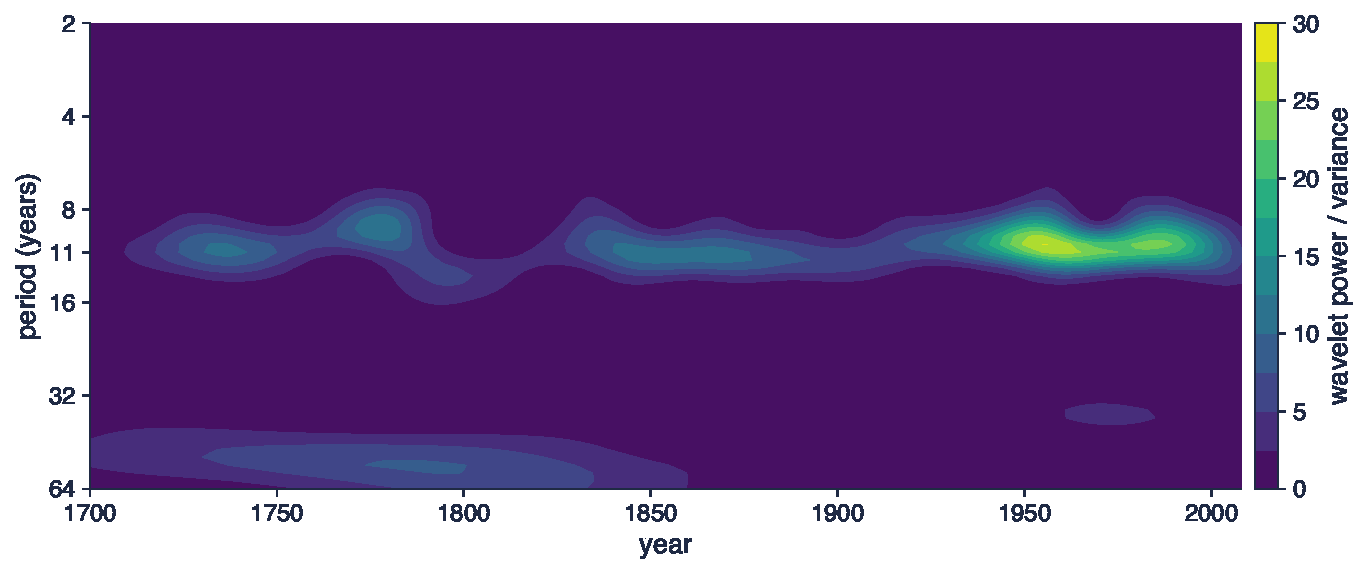
\includegraphics[width=0.97\textwidth,height=0.56\textheight,keepaspectratio]{tsa_ch12_wavelet.pdf}
\end{center}
\vspace{-0.25cm}
\begin{itemize}
    \item Morlet wavelet power of the standardised yearly sunspot numbers, 1700--2008, periods 2 to 64 years; bright colours mean high power
\end{itemize}
\quantlet{TSA\_ch12\_wavelet}{\qlurl{TSA_ch12_wavelet}}
\end{frame}

\begin{frame}{Interpreting the scalogram}
\itemsize{\small}
\begin{itemize}
    \item The 11-year band is present throughout, but its strength changes
    \begin{itemize}
        \item average power in the 8--14-year band: 2.0 in 1795--1830 (the weak Dalton minimum) against 5.7 over the whole sample; the maximum is around 1956
    \end{itemize}
    \item The periodogram averaged these changes into one peak; the scalogram shows when the cycle was strong or weak
    \item Edges of the chart are less reliable (the wavelet runs out of data): this region is called the cone of influence
\end{itemize}
\end{frame}

\begin{frame}{Recap: Long memory, filters, two series, wavelets}
\itemsize{\small}
\begin{itemize}
    \item Long memory is a pole at $\nu = 0$: slope $-2d$ on a log--log plot (GPH)
    \item A filter multiplies the spectrum by its squared gain: differencing and the HP filter reshape cycles
    \item Coherence is a correlation by frequency; the phase gives the lead or the lag
    \item Wavelets show how cycles change over time
\end{itemize}
\end{frame}


%=============================================================================
\section{Possible contribution of AI}
%=============================================================================

\begin{frame}{Possible contribution of AI}
\itemsize{\small}
\begin{itemize}
    \item \textbf{Code}
    \begin{itemize}
        \item a first draft of a periodogram, a Daniell smoother, a Welch estimate or a coherence plot
    \end{itemize}
    \item \textbf{Explanation}
    \begin{itemize}
        \item a second explanation of leakage, aliasing or the bias--variance trade-off of the bandwidth
    \end{itemize}
    \item \textbf{Exploration}
    \begin{itemize}
        \item spectra of many series at once (load of several countries, GDP of all EU members) and a first reading of the peaks
    \end{itemize}
    \item Example prompt
    \begin{itemize}
        \item \aiprompt{Write Python code that reads hourly electricity load, removes the mean, computes the periodogram with a Hann taper and a Welch estimate with 8-week segments, plots both on a log-log scale against the period in hours, and marks 24, 12 and 168 hours.}
    \end{itemize}
\end{itemize}
\end{frame}

\begin{frame}{Checks you must run}
\itemsize{\small}
\begin{itemize}
    \item The units: frequency in cycles per observation or radians; \texttt{scipy.signal.welch} returns a one-sided density (twice our $f$)
    \item The period: $1/\nu$ in observations; convert to years, quarters or hours yourself
    \item Parseval: the ordinates must add up to $T$ times the variance; test the code on a cosine with a known frequency
    \item A peak is a cycle only with a test or a confidence band; a raw periodogram always has tall spikes
    \item Trends, breaks and filters create low-frequency power and false peaks: check the data and the transformation first
    \item Every cited reference: it must exist; check the DOI
\end{itemize}
\end{frame}


%=============================================================================
\section{Summary}
%=============================================================================

\begin{frame}{Key takeaways}
\itemsize{\small}
\begin{itemize}
    \item The spectrum splits the variance of a stationary series by frequency; it carries the same information as the ACF
    \item Read its shape: flat (white noise), falling (persistence), peaked (cycles), a pole at zero (long memory)
    \item The raw periodogram is unbiased but inconsistent: taper, smooth and add confidence bands
    \item Real cycles: 11 years in sunspots, 4--8 years in GDP, 24 hours and 1 week in electricity load
    \item Filters reshape spectra; coherence and phase relate the cycles of two series
\end{itemize}
\end{frame}

\begin{frame}{Key formulas}
\itemsize{\small}
{\renewcommand{\arraystretch}{1.35}\begin{center}
\scriptsize
\begin{tabular}{ll}
\toprule
\textbf{Quantity} & \textbf{Formula} \\
\midrule
Spectral density & $f(\nu) = \sum_h\gamma(h)e^{-2\pi i\nu h}$, \quad $\gamma(0) = \int_{-1/2}^{1/2} f(\nu)\,d\nu$ \\
AR(1), MA(1) & $\sigma^2/(1 - 2\phi\cos 2\pi\nu + \phi^2)$, \quad $\sigma^2(1 + 2\theta\cos 2\pi\nu + \theta^2)$ \\
ARMA & $\sigma^2|\theta(e^{-2\pi i\nu})|^2/|\phi(e^{-2\pi i\nu})|^2$ \\
Periodogram & $I(\nu_j) = |T^{-1/2}\sum_t x_t e^{-2\pi i\nu_j t}|^2$, \quad $\nu_j = j/T$, \quad $2I/f \approx \chi^2_2$ \\
Daniell & $\hat f(\nu_j) = \frac1L\sum_{|k| \le m} I(\nu_{j+k})$, \quad $L = 2m + 1$, \quad $B = L/T$ \\
95\% band & $[2L\hat f/\chi^2_{2L}(0.975),\ 2L\hat f/\chi^2_{2L}(0.025)]$ \\
Linear filter & $f_y(\nu) = |A(\nu)|^2 f_x(\nu)$, \quad $|1 - e^{-2\pi i\nu}|^2 = 4\sin^2(\pi\nu)$ \\
Coherence, phase & $\rho^2_{xy} = |f_{xy}|^2/(f_x f_y)$, \quad $\varphi = \arg f_{xy}$, \quad lag $= |\varphi|/(2\pi\nu)$ \\
\bottomrule
\end{tabular}
\end{center}
}
\end{frame}

\begin{frame}{Self-assessment (1/2)}
\itemsize{\footnotesize}
\begin{itemize}
    \item \textbf{Question}: weekly data show a peak at $\nu = 0.0192$. What is the period?
    \begin{itemize}
        \item \textbf{Answer}: $1/0.0192 \approx 52$ weeks: an annual cycle
    \end{itemize}
    \item \textbf{Question}: what are $f(0)$ and $f(1/2)$ of an AR(1) with $\phi = -0.5$, $\sigma^2 = 1$?
    \begin{itemize}
        \item \textbf{Answer}: $f(0) = 1/1.5^2 = 0.44$ and $f(1/2) = 1/0.5^2 = 4$: power at high frequencies
    \end{itemize}
    \item \textbf{Question}: why does a longer sample not make the raw periodogram more precise?
    \begin{itemize}
        \item \textbf{Answer}: each ordinate still has variance about $f^2$; more data only adds ordinates; precision needs averaging
    \end{itemize}
    \item \textbf{Question}: with $L = 5$, how wide is the 95\% band relative to $\hat f$?
    \begin{itemize}
        \item \textbf{Answer}: from 0.49 to 3.08 times $\hat f$ ($df = 10$)
    \end{itemize}
\end{itemize}
\end{frame}

\begin{frame}{Self-assessment (2/2)}
\itemsize{\footnotesize}
\begin{itemize}
    \item \textbf{Question}: a monthly series observed only every second month has a 3-month cycle. Where does it appear?
    \begin{itemize}
        \item \textbf{Answer}: $\nu = 2/3$ cycles per two months is above $1/2$; it folds to $1/3$: a false cycle of 3 observations, i.e.\ 6 months
    \end{itemize}
    \item \textbf{Question}: what does the first difference do to a cycle of 40 quarters?
    \begin{itemize}
        \item \textbf{Answer}: it multiplies its power by $4\sin^2(\pi/40) = 0.025$: the cycle almost disappears
    \end{itemize}
    \item \textbf{Question}: the log--log periodogram of a series has slope $-0.6$ near zero. What is $d$?
    \begin{itemize}
        \item \textbf{Answer}: slope $= -2d$, so $d = 0.3$: stationary long memory (\tsachlink{https://danpele.github.io/Time-Series-Analysis/EN/Courses/chapter8_long_memory_arfima.pdf}{Chapter 8})
    \end{itemize}
    \item \textbf{Question}: the squared coherence of two series is 0.9 at 5-year cycles and 0.1 at monthly cycles. What does it mean?
    \begin{itemize}
        \item \textbf{Answer}: their business cycles move together; their short-run noise does not
    \end{itemize}
    \item Next: \tsachlink{https://danpele.github.io/Time-Series-Analysis/EN/Courses/chapter13_bubbles_lppl.pdf}{Chapter 13}, speculative bubbles and LPPL models
\end{itemize}
\end{frame}


%=============================================================================
\section{References}
%=============================================================================

\begin{frame}{References (1/2)}
\itemsize{\tiny}
\begin{itemize}
    \item Bartlett, M. S. (1950). Periodogram analysis and continuous spectra. \textit{Biometrika}, 37(1--2), 1--16. \href{https://doi.org/10.1093/biomet/37.1-2.1}{doi:10.1093/biomet/37.1-2.1}
    \item Baxter, M., \& King, R. G. (1999). Measuring business cycles: Approximate band-pass filters for economic time series. \textit{Review of Economics and Statistics}, 81(4), 575--593. \href{https://doi.org/10.1162/003465399558454}{doi:10.1162/003465399558454}
    \item Blackman, R. B., \& Tukey, J. W. (1958). The measurement of power spectra from the point of view of communications engineering, Part I. \textit{Bell System Technical Journal}, 37(1), 185--282. \href{https://doi.org/10.1002/j.1538-7305.1958.tb03874.x}{doi:10.1002/j.1538-7305.1958.tb03874.x}
    \item Brockwell, P. J., \& Davis, R. A. (1991). \textit{Time Series: Theory and Methods} (2nd ed.). Springer. \href{https://doi.org/10.1007/978-1-4419-0320-4}{doi:10.1007/978-1-4419-0320-4}
    \item Cooley, J. W., \& Tukey, J. W. (1965). An algorithm for the machine calculation of complex Fourier series. \textit{Mathematics of Computation}, 19(90), 297--301. \href{https://doi.org/10.1090/S0025-5718-1965-0178586-1}{doi:10.1090/S0025-5718-1965-0178586-1}
    \item Fisher, R. A. (1929). Tests of significance in harmonic analysis. \textit{Proceedings of the Royal Society of London, Series A}, 125(796), 54--59. \href{https://doi.org/10.1098/rspa.1929.0151}{doi:10.1098/rspa.1929.0151}
    \item Geweke, J., \& Porter-Hudak, S. (1983). The estimation and application of long memory time series models. \textit{Journal of Time Series Analysis}, 4(4), 221--238. \href{https://doi.org/10.1111/j.1467-9892.1983.tb00371.x}{doi:10.1111/j.1467-9892.1983.tb00371.x}
    \item Granger, C. W. J. (1966). The typical spectral shape of an economic variable. \textit{Econometrica}, 34(1), 150--161. \href{https://doi.org/10.2307/1909859}{doi:10.2307/1909859}
    \item Hamilton, J. D. (1994). \textit{Time Series Analysis}. Princeton University Press. \href{https://doi.org/10.1515/9780691218632}{doi:10.1515/9780691218632}
\end{itemize}
\end{frame}

\begin{frame}{References (2/2)}
\itemsize{\tiny}
\begin{itemize}
    \item Hamilton, J. D. (2018). Why you should never use the Hodrick--Prescott filter. \textit{Review of Economics and Statistics}, 100(5), 831--843. \href{https://doi.org/10.1162/rest_a_00706}{doi:10.1162/rest\_a\_00706}
    \item Hodrick, R. J., \& Prescott, E. C. (1997). Postwar U.S. business cycles: An empirical investigation. \textit{Journal of Money, Credit and Banking}, 29(1), 1--16. \href{https://doi.org/10.2307/2953682}{doi:10.2307/2953682}
    \item Huang, C., \& Petukhina, A. (2022). \textit{Applied Time Series Analysis and Forecasting with Python}. Springer. \href{https://doi.org/10.1007/978-3-031-13584-2}{doi:10.1007/978-3-031-13584-2}
    \item Schuster, A. (1898). On the investigation of hidden periodicities with application to a supposed 26 day period of meteorological phenomena. \textit{Terrestrial Magnetism}, 3(1), 13--41. \href{https://doi.org/10.1029/TM003i001p00013}{doi:10.1029/TM003i001p00013}
    \item Shumway, R. H., \& Stoffer, D. S. (2017). \textit{Time Series Analysis and Its Applications: With R Examples} (4th ed.). Springer. \href{https://doi.org/10.1007/978-3-319-52452-8}{doi:10.1007/978-3-319-52452-8}
    \item Torrence, C., \& Compo, G. P. (1998). A practical guide to wavelet analysis. \textit{Bulletin of the American Meteorological Society}, 79(1), 61--78. \href{https://doi.org/10.1175/1520-0477(1998)079<0061:APGTWA>2.0.CO;2}{doi:10.1175/1520-0477(1998)079<0061:APGTWA>2.0.CO;2}
    \item Welch, P. D. (1967). The use of fast Fourier transform for the estimation of power spectra: A method based on time averaging over short, modified periodograms. \textit{IEEE Transactions on Audio and Electroacoustics}, 15(2), 70--73. \href{https://doi.org/10.1109/TAU.1967.1161901}{doi:10.1109/TAU.1967.1161901}
    \item Yule, G. U. (1927). On a method of investigating periodicities in disturbed series, with special reference to Wolfer's sunspot numbers. \textit{Philosophical Transactions of the Royal Society of London, Series A}, 226, 267--298. \href{https://doi.org/10.1098/rsta.1927.0007}{doi:10.1098/rsta.1927.0007}
\end{itemize}
\end{frame}

\end{document}
